\documentclass[final, 12pt,oneside]{class_diss}
\usepackage{titlesec}
\titleformat{\chapter}[display]
  {\normalfont\bfseries}{}{0pt}{\Large}

% +--------------------------------------------------------------------+
% | The following command sets the bibliography style to American
% | Institute of Physics (AIP).  Other styles are available in the
% | styles directory.  To use a different style, replace "aip" with
% | the filename of the style you want to use.
% +--------------------------------------------------------------------+

\bibliographystyle{alpha}

\usepackage[utf8]{inputenc}
\usepackage[T1]{fontenc}
\usepackage[spanish]{babel}
% +--------------------------------------------------------------------+
% | Now, we add in all external packages that we will use throughout   |
% | the document.  You can add other packages as needed.
% +--------------------------------------------------------------------+

%\usepackage{caption} % Customize captions a bit more
\usepackage{amsmath,amsthm,amssymb} % American Mathematics Society standards
\usepackage{algorithm} 
\usepackage[noend]{algpseudocode}
\floatname{algorithm}{Algoritmo}
\renewcommand{\listalgorithmname}{Lista de algoritmos}
\renewcommand{\algorithmicrequire}{\textbf{Entrada:}}
\renewcommand{\algorithmicensure}{\textbf{Salida:}}
\renewcommand{\algorithmicend}{\textbf{fin}}
\renewcommand{\algorithmicif}{\textbf{si}}
\renewcommand{\algorithmicthen}{\textbf{ }}
\renewcommand{\algorithmicelse}{\textbf{en otro caso}}
\renewcommand{\algorithmicreturn}{\textbf{devolver }}

 % archivo de traduccion
\usepackage{listings}

\lstset{basicstyle=\fontsize{10}{12}\selectfont\ttfamily,
        framerule=0pt,frame=single, %frame=trBL,frameround=ftttm,
        lineskip=0pt,
        emptylines=1,
        showstringspaces=false,
        escapechar=·,
        language=Python
}

\usepackage{lmodern} %Vectorial source
%\usepackage{wrapfig} % Wraps text around a figure or table
\usepackage{graphicx} % Extended graphics package.
\usepackage{subfig}
\usepackage{float}
%\usepackage{fancyhdr} % Efficiently handles headers and footers
%\usepackage{braket} % Bra-Ket notation package
%\usepackage{mathrsfs} % Specialized Math fonts (Hamiltonian, etc.)
%\usepackage{boxedminipage} % Boxed text can be produced
%\usepackage{setspace} % Controls line spacing via \begin{space}
\usepackage{amsxtra}
\usepackage{latexsym}


% +--------------------------------------------------------------------+
% | The color package allows one to select colors for hyperlinking     |
% | (see below).                                                       |
% +--------------------------------------------------------------------+

\usepackage[usenames]{color}

% +--------------------------------------------------------------------+
% | Colors defined for use with this template.                         |
% +--------------------------------------------------------------------+

\definecolor{  Pink}{rgb}{1.0, 0.5, 0.5}
\definecolor{Maroon}{rgb}{0.8, 0.0, 0.0}

% +--------------------------------------------------------------------+
% | In the commands below, we use the 'natbib' package, and specify    |
% | the 'sort&compress' option, which condenses                        |
% | citations from (1,2,3,5,9,10,11) to (1-3,5,9-11).  The 'bibpunct'  |
% | option selects various parameters for how the citation will be     |
% | displayed.  In this case, only the comma (separation between       |
% | citations) and the 's' (superscript) arguments are chosen.  The    |
% | other curly braces deal with how to 'wrap' the citation (using     |
% | parentheses, brackets, etc.) and are not needed for the chosen     |
% | style.                                                             |
% +--------------------------------------------------------------------+

\usepackage{natbib}
%\bibpunct{}{}{,}{s}{}{}
%\usepackage{hypernat}

% +--------------------------------------------------------------------+
% | Theorems, observations, lemmas       
% +--------------------------------------------------------------------+

\newtheorem{remark}{Observación}[chapter]
\newtheorem{theorem}{Teorema}[chapter]
\newtheorem{lemma}{Lema}[chapter]
\newtheorem{definition}{Definición}[chapter]

% +--------------------------------------------------------------------+
% | Lastly, the hyperref package allows one to hyperlink cross-        |
% | references and figures in a LaTeX document.                        |
% +--------------------------------------------------------------------+

\usepackage[pdftex, plainpages=false]{hyperref}

\hypersetup{
    linktocpage=true,
    colorlinks=true,
    citecolor=blue,
    urlcolor=red,
    linkcolor=Maroon,
    citebordercolor={1 0 0},
    urlbordercolor={1 0 0},
    linkbordercolor={.7 .8 .8},
    breaklinks=true
    }

% +--------------------------------------------------------------------+
% | Page margins are set on 1 inch on all sides.                       |
% +--------------------------------------------------------------------+

\topmargin      = -0.56in
\textheight     =  8.60in
\textwidth      =  6.46in
\oddsidemargin  =  0.02in


\def\lcomen#1{\footnote{{\color{red}Comentario de Luis:} #1}}

% +--------------------------------------------------------------------+
% | The document finally begins here.                                  |
% +--------------------------------------------------------------------+

\begin{document}


  \setcounter{page}{1}


% +--------------------------------------------------------------------+
% | Title Page -- Required for both Doctoral and Masters Students
% +--------------------------------------------------------------------+

%% +--------------------------------------------------------------------+
% | Title Page
% +--------------------------------------------------------------------+

\newpage

% +--------------------------------------------------------------------+
% | This page should not contain a page number.  We use the
% | \thispagestyle[empty] command below to suppress page numbers
% | and other style elements.
% +--------------------------------------------------------------------+

\thispagestyle{empty}

% +--------------------------------------------------------------------+
% | The Title page begins here.
% +--------------------------------------------------------------------+

\begin{center}

   \vspace{1cm}

% +--------------------------------------------------------------------+
% | On the line below, replace "ENTER YOUR TITLE" with the title of
% | your ETDR.  Use all CAPITAL LETTERS.
% +--------------------------------------------------------------------+

   {\Large El protocolo blockchain y su aplicación en entornos distribuidos.}\\

   \vspace{0.5cm}



   \vspace{0.5cm}



   {\large Luis Alberto Glaría Silva}\\

   \vspace{0.5cm}




   GRADO EN MATEMÁTICAS. FACULTAD DE CIENCIAS MATEMÁTICAS\\
   UNIVERSIDAD COMPLUTENSE DE MADRID \\


   \vspace{0.65cm}
   \rule{2in}{0.5pt}\\
   \vspace{0.85cm}

  
\includegraphics[height=2in]{figures/escudo.jpg}
  

%+-- Escribe el nombre de tu asignatura de fin de grado o master (Ingeniería de matemáticas,....)
   \vspace{0.5cm}
Trabajo de Fin de Grado

   \vspace{0.5cm}





% +--------------------------------------------------------------------+
%  Fecha 
% +--------------------------------------------------------------------+

  Julio de 2019\\
   \vspace{1cm}

\end{center}

{\raggedleft
Director:\\
   \vspace{ 1cm}
Luis Llana Díaz\\

}


% +--------------------------------------------------------------------+
% | Use the section below if you have co-major professors.
% +--------------------------------------------------------------------+

%\begin{flushleft}
%   \hspace{10cm}Approved by:\\
%   \vspace{ 1cm}
%   \hspace{10cm}Co-Major Professor\\
%   \hspace{10cm}Enter Your Co-Major Professor's Name\\
%   \vspace{.5cm}
%   \hspace{10cm}Co-Major Professor\\
%   \hspace{10cm}Enter Your Co-Major Professor's Name\\
%\end{flushleft}

%   \pdfbookmark[0]{Portada}{PDFPortadaPage}

% +--------------------------------------------------------------------+
% | Autorizacion Page -- Required for both Doctoral and Masters Students
% +--------------------------------------------------------------------+

%% +--------------------------------------------------------------------+
% | Copyright Page
% +--------------------------------------------------------------------+

\newpage

\thispagestyle{empty}

\begin{center}

{\bf \Huge Autorización de difusión}

\vspace{1cm}

% +--------------------------------------------------------------------+
% | On the line below, replace "Enter Your Name" with your name
% | Use the same form of your name as it appears on your title page.
% | Use mixed case, for example, Lori Goetsch.
% +--------------------------------------------------------------------+

   \large Autor\\

   \vspace{0.5cm}

% +--------------------------------------------------------------------+
% | On the line below, replace Fecha
% |
% +--------------------------------------------------------------------+

   Fecha\\

   \vspace{0.5cm}
   \end{center}
   
El/la abajo firmante, matriculado/a en el Máster en Investigación en Informática de la Facultad de Informática, autoriza a la Universidad Complutense de Madrid (UCM) a difundir y utilizar con fines académicos, no comerciales y mencionando expresamente a su autor el presente Trabajo Fin de Máster: “TÍTULO”, realizado durante el curso académico 20XX-20XX bajo la dirección de XXXX [y con la colaboración externa de dirección de YYYY] en el Departamento de XXXX, y a la Biblioteca de la UCM a depositarlo en el Archivo Institucional E-Prints Complutense con el objeto de incrementar la difusión, uso e impacto del trabajo en Internet y garantizar su preservación y acceso a largo plazo.


%   \pdfbookmark[0]{Autorización}{PDFAutorizacionPage}

% +--------------------------------------------------------------------+
% | Resumen y astract
% +--------------------------------------------------------------------+
   
%   % +--------------------------------------------------------------------+
% | Copyright Page
% +--------------------------------------------------------------------+

\newpage

\thispagestyle{empty}

\begin{center}

{\bf \Huge Resumen}

  \end{center}
\vspace{1cm}

Desde la creación del Bitcoin en 2008 y del crecimiento de las inversiones en criptomonedas a partir de 2012, el protocolo Blockchain ha ido despertando cada vez más interés por sus posibles aplicaciones en diversos campos.

En este trabajo nos alejaremos de las cuestiones económicas relacionadas con las criptomonedas para por un lado analizar los fundamentos matemáticos de esta tecnología y por otro lado ver la relación de este protocolo con ciertos problemas de la programación distribuida. Para ello se estudia el funcionamiento y corrección de una posible especificación del Blockchain. También se ha hecho una implementación de este protocolo donde se han podido llevar a la práctica algunas ideas desarrolladas en el trabajo.
%Una de las tecnologías que han despertado un mayor interés recientemente es el blockchain.

%En cada uno de los capítulos de este trabajo se tocará 
\vspace{1cm}

% +--------------------------------------------------------------------+
% | On the line below, repla	ce Fecha
% |
% +--------------------------------------------------------------------+

\begin{center}

{\bf \Large Palabras clave}

   \end{center}

   \vspace{0.5cm}
   
   Blockchain, Criptografía de clave pública, Bitcoin, Funciones Hash, Consenso, Prueba de trabajo, Sistemas distribuidos.
   





   
%   \pdfbookmark[0]{Resumen}{PDFResumenPage}

%    % +--------------------------------------------------------------------+
% | Copyright Page
% +--------------------------------------------------------------------+

\newpage

\thispagestyle{empty}

\begin{center}

{\bf \Huge Abstract}

  \end{center}
\vspace{1cm}

Since the creation of Bitcoin in 2008, and the growth of investments in crypto-currencies in 2012, the Blockchain protocol has created a great interest for its possible applications in various fields.

This paper will focus on the mathematical foundations of this technology and it's relation to certain problems of distributed programming  rather than in the economic features of crypto-currencies. In order to achieve this objective the operation and correctness of a possible Blockchain specification is studied. An implementation of Blockchain was created, where it was possible to develop in practice some ideas of this document.
\vspace{1cm}

% +--------------------------------------------------------------------+
% | On the line below, replace Fecha
% |
% +--------------------------------------------------------------------+

\begin{center}

{\bf \Large Keywords}

   \end{center}

   \vspace{0.5cm}
   
   Blockchain, public-key cryptography, Bitcoin, Hash functions, consensus protocol, proof of work, distributed systems.
   



   



%       \pdfbookmark[0]{Abstract}{PDFAbstractPage}
%    \vfill


% +--------------------------------------------------------------------+
% | We use the following code to suppress page numbers and other
% | style issues we do not want present on a given page.               |
% +--------------------------------------------------------------------+

%\thispagestyle{empty} Looks like it's ok to remove this line
\newpage
\pagenumbering{roman}

% +--------------------------------------------------------------------+
% | On the line below, set the number to represent the page number of
% | the Table of Contents page.  For example, if the Table of Contents
% | page is the 8th page of your document, enter 8 in the brackets.  This
% | number may vary, depending on the length of your abstract.
% |
% | Numbers do not appear on the title and abstract pages, but they are
% | included in the page count.  The Table of Contents page is the
% | first page on which page numbers are displayed.
% +--------------------------------------------------------------------+

\setcounter{page}{1}

% +--------------------------------------------------------------------+
% | Here, we will generate our Table of Contents (TOC) entries.        |
% | This adds the section to the TOC and then generates the indicated  |
% | section.                                                           |
% +--------------------------------------------------------------------+

\phantomsection
\addcontentsline{toc}{chapter}{Índice}

\tableofcontents
%\listoffigures
%\listoftables

%\hfill  Are these lines necessary?
%\hfill

% +--------------------------------------------------------------------+
% | Acknowledgements Page
% |
% | If you choose not to have an Acknowledgements page, comment out
% | or delete the following 3 lines.
% +--------------------------------------------------------------------+

%% +--------------------------------------------------------------------+
% | Acknowledgements Page (Optional)                                   |
% +--------------------------------------------------------------------+

\newpage
\begin{center}
{\bf \Huge Agradecimientos}
\end{center}
\vspace{1cm}
\setlength{\baselineskip}{0.8cm}

%\pdfbookmark[0]{Acknowledgements}{PDF_Acknowledgements}

% +--------------------------------------------------------------------+
% | Enter text for your acknowledgements in the space below this box.  |
% |                                                                    |
% +--------------------------------------------------------------------+

Agradecimientos.....

%\phantomsection
%\addcontentsline{toc}{chapter}{Agradecimientos}

% +--------------------------------------------------------------------+
% | Dedication Page
% |
% | If you choose not to have a Dedication page, comment out
% | or delete the following 3 lines.
% +--------------------------------------------------------------------+

%% +--------------------------------------------------------------------+
% | Dedication Page (Optional)
% +--------------------------------------------------------------------+

\newpage
\begin{center}
{\bf \Huge Dedicatoria}
\end{center}
\vspace{1cm}
\setlength{\baselineskip}{0.8cm}

%\pdfbookmark[0]{Dedication}{PDF_Dedication}

% +--------------------------------------------------------------------+
% | Enter the text for your dedication in the space below this box.
% +----------------
Texto...
%\phantomsection
%\addcontentsline{toc}{chapter}{Dedicatoria}

% +--------------------------------------------------------------------+
% | Preface Page
% +--------------------------------------------------------------------+

%% +--------------------------------------------------------------------+
% | Preface (Optional)
% +--------------------------------------------------------------------+

\newpage
\begin{center}
{\bf \Huge Preface}
\end{center}
\vspace{1cm}
\setlength{\baselineskip}{0.8cm}

%\pdfbookmark[0]{Preface}{PDF_Preface}

% +--------------------------------------------------------------------+
% | Enter text of your Preface in the space below this box.
% +--------------------------------------------------------------------+

This template uses a separate file for each section of your ETDR:
title page, abstract, preface, chapters, reference, etc.  This
makes it easier to organize and work with a lengthy document.  The
template is configured with page margins required by the Graduate
School and will automatically create a table of contents, lists of
tables and figures, and PDF bookmarks.

Although the template gives you a foundation for creating your
ETDR, you will need a working knowledge of LaTeX in order to
produce a final document.  You should be familiar with LaTeX
commands for formatting text, equations, tables, and other
elements you will need to include in your ETDR.

This template uses a separate file for each section of your ETDR:
title page, abstract, preface, chapters, reference, etc.  This
makes it easier to organize and work with a lengthy document.  The
template is configured with page margins required by the Graduate
School and will automatically create a table of contents, lists of
tables and figures, and PDF bookmarks.

Although the template gives you a foundation for creating your
ETDR, you will need a working knowledge of LaTeX in order to
produce a final document.  You should be familiar with LaTeX
commands for formatting text, equations, tables, and other
elements you will need to include in your ETDR.

This template uses a separate file for each section of your ETDR:
title page, abstract, preface, chapters, reference, etc.  This
makes it easier to organize and work with a lengthy document.  The
template is configured with page margins required by the Graduate
School and will automatically create a table of contents, lists of
tables and figures, and PDF bookmarks.

Although the template gives you a foundation for creating your
ETDR, you will need a working knowledge of LaTeX in order to
produce a final document.  You should be familiar with LaTeX
commands for formatting text, equations, tables, and other
elements you will need to include in your ETDR.

%\phantomsection
%\addcontentsline{toc}{chapter}{Preface}

% +--------------------------------------------------------------------+
% | We use arabic (1, 2, 3...) page numbering starting from page 1.    |
% | Note, however, that there are many pages where this is not the     |
% | desired behavior - such as the Title page, or abstract.  In these  |
% | cases, we can use \thispagestyle{empty} to suppress page numbers,  |
% | and other general style issues that we've defined globally.        |
% +--------------------------------------------------------------------+

\newpage
\pagenumbering{arabic}
\setcounter{page}{1}

% +--------------------------------------------------------------------+
% | Here is where we include individual sections of the thesis or
% | dissertation.                                                      |
% +--------------------------------------------------------------------+

% +--------------------------------------------------------------------+
% | Chapters
% +--------------------------------------------------------------------+

% +--------------------------------------------------------------------+
% | Sample Chapter
% +--------------------------------------------------------------------+

\cleardoublepage



\chapter{Introducción y objetivos.}
\label{introduccion}

%explicar aqui el problema del doble gasto
En 1969 el Departamento de Defensa de los Estados Unidos instaló los primeros nodos de la \textit{Advanced Research Projects Agency Network} (ARPANET), precursora de la actual Internet. Desde este momento surgió la necesidad de garantizar las comunicaciones entre varias computadoras incluso en el supuesto en que algunas de ellas dejaran de funcionar, o se interrumpieran parte de las conexiones que hacían posible la transmisión de información\citep{arpanet}. Nacen así las redes de ordenadores y con ellas el concepto de sistemas distribuidos.

Desde este momento surgieron diversas aplicaciones y protocolos, tales como Napster, Gnutella o Bittorrent \citep{redes_p2p}, que buscaban resolver diferentes problemas de forma cooperativa y distribuida. El sector financiero no estuvo ajeno a estas transformaciones, y ya desde 1983 se teorizó sobre la posibilidad de de utilizar monedas digitales, aunque requiriendo de cierta entidad central que validara las operaciones \citep{chaum1983blind}. También surgió la idea con B-Money \citep{b_money} de utilizar una moneda digital completamente descentralizada, pero esta propuesta no llegó a ser implementada.


 %A este registro lo llamaremos cadena de bloques para distinguirlo del nombre del protocolo.
%aquí poner algo de la historia del protocolo, hablar del blockchain y de las distintas versiones (fundamentalmente criptomonedas) así enlazo con lo ya escrito.

En el año 2008, con la publicación del artículo \textit{Bitcoin: A Peer-to-Peer Electronic Cash System} \citep{bitcoin}, nace el protocolo Blockchain. Se desconoce la verdadera identidad de la persona u organización oculta bajo el seudónimo de Satoshi Nakamoto, autor de este documento. %\footnote{https://bitcoin.org/bitcoin.pdf}
En el año 2009, el propio Nakamoto publicó el código, escrito en C++, de la criptomoneda Bitcoin. Posteriormente fueron creadas nuevas monedas digitales basadas en la idea original del Bitcoin y a partir del año 2014 se comenzaron a estudiar aplicaciones del Blockchain distintas de las criptomonedas.

Se puede definir entonces al Blockchain como un protocolo que permite mantener un registro distribuido e inmutable de las transacciones o comunicaciones entre los participantes de una determinada red. Y que para garantizar en todo momento que la información almacenada es veraz, se tiene también un mecanismo de consenso que no necesita de ningún tipo de centralización para funcionar. En este punto conviene hacer un apunte sobre la terminología usada, aunque en la literatura se suele utilizar \textit{blockchain} en minúsculas para hacer referencia al registro donde se almacena la información y reservar \textit{Blockchain} para hacer referencia a la tecnología o al protocolo, en este trabajo utilizaremos la traducción al español: \textit{cadena de bloques} cuando se haga referencia a la estructura que conforma la base de datos.

Una aspecto importante de las primeras criptomonedas es su carácter completamente público: cualquier usuario de internet podía unirse a la red y participar activamente sin necesidad de ninguna autorización o verificación. 

Todas estas implementaciones, independientemente de las variaciones en el protocolo, tienen en común el carácter distribuido del algoritmo y la inmutabilidad del registro (cadena de bloques). Sin embargo, se pueden establecer 3 distinciones generales en base a como se trate el aspecto público y el nivel de  descentralización \citep{type_blockchain}:
\begin{itemize}
\item \textit{Blockchain público:} Cualquiera puede unirse a la red, todos los nodos pueden leer el registro, realizar transacciones y participar en el consenso.
\item \textit{Blockchain de consorcio:} En el algoritmo de consenso solo intervienen una parte de los nodos. El acceso a la red y las consultas al registro en principio están abiertas a todos. Este sería el caso de una red pública y centralizada.
\item \textit{Blockchain privado:} El acceso a la red no es público y además tanto la lectura del registro como la participión en el algoritmo de consenso pueden encontrarse limitados. Estamos ante una red privada que puede estar en mayor o menor medida centralizada.
\end{itemize}

%Debe notarse que la frontera entre un protocolo blockchain de consorcio y uno privado son más bien difusas
Dado que es la variante más conocida y utilizada, y es a la que pertenece la primera criptomoneda, el Bitcoin, en este trabajo nos centraremos fundamentalmente en el Blockchain de tipo público. 


Al igual que no existe una única alternativa en la elección de los niveles de centralización y privacidad, el mecanismo utilizado para alcanzar un acuerdo entre los participantes en la red (consenso) difiere entre las diferentes implementaciones del Blockchain. Sin embargo, para explicar las diferencias entre cada uno de estos algoritmos se deben definir y estudiar ciertas cuestiones referentes a la criptografía.% y curvas algebraicas.

Será por tanto el primer objetivo de este trabajo dar las nociones matemáticas básicas que fundamentan el Blockchain. De eso tratará el capítulo \ref{cap1}. Una vez sea posible justificar parte del marco teórico de esta tecnología el siguiente paso será explicar su funcionamiento, tarea que será realizada en el tema \ref{cap3}. En este punto se explicarán de forma más extensa las diferencias entre algunas de las diferentes implementaciones de este protocolo existentes que han sido mencionadas de forma somera en esta introducción. Hay que tener en cuenta que el desarrollo de este protocolo ha estado estrechamente ligado a las distintas implementaciones del mismo (o más bien al éxito de estas) y no tanto a un trabajo teórico sistemático. 

Un tercer objetivo consistirá en estudiar el Blockchain dentro del contexto específico de la computación distribuida y de la resolución de uno de los problemas fundamentales de este campo. Sobre este asunto versará el tema \ref{cap4}. Para finalizar, se realizará en el capítulo \ref{implementacion} una implementación del Blockchain en la que se podrá comprobar que es posible llevar a la práctica, de forma relativamente sencilla, las ideas desarrolladas en este trabajo.

%Más allá del interés socioeconómico que puedan despertar las criptomonedas el blockchain constituye una potente herramienta dentro de la programación distribuida

%siempre que garanticen que la información que cada nodo pretende escribir en el registro es considerada cierta por una parte significativa (quorum) de los otros nodos. Una característica de las primeras implementaciones del protocolo blockchain es que estaban pensadas para trabajar con grandes cantidades de participantes, por tanto es infactible que el quorum sea toda la red.

%hablar de proof of work, algoritmos de consenso, y porque para las criptos se usan estos y no por ejemplo raft y demás. Ver por que no se pueden usar raft y paxos para blockchain (esto quizas iria mejor en otro tema)
%revisar en el primer parrafo del capitulo lo que se dice de este algoritmo
%meter aqui algo del problema de los generales bizantinos, explicar el problema y demás, y decir que sobre esto se volverá al final del trabajo.
%no entrar en mucho detalle, en siguientes capítulos esto se tocará más.








% +--------------------------------------------------------------------+
% | Uncomment the lines below to add additional chapters.  Name the
% | files chapter2.tex for Chapter 2, chapter3.tex for Chapter 3, etc.
% +--------------------------------------------------------------------+

% +--------------------------------------------------------------------+
% | Sample Chapter 2
% +--------------------------------------------------------------------+

\cleardoublepage

\chapter{Criptografía y Blockchain}
\label{cap1}
%En este capitulo trataremos todo lo referente a protocolos criptograficos aplicados en blockchain.

%secciones: una breve introduccion sobre lo que se pretende con la criptografia, ecdsa: curvas elipticas, algoritmo de consenso, coste computacional de los algoritmos, quizás algun extra tipo implementacion...
%\section{Criptografía de clave pública} no poner como seccion, sino incluirlo en la introduccion del capitulo
Garantizar la autenticidad de las transacciones entre los nodos y la integridad del registro es la tarea de la criptografía dentro del blockchain. La criptografía de clave pública, donde no es necesario la existencia de un canal seguro para transmitir la información, es el método criptográfico utilizado en el Blockchain, pues justamente en este entorno público toda la información transmitida es vista por los demás participantes.
Este método, desarrollado en la década del 70 del siglo XX, solucionó algunas limitaciones de la criptografía de clave simétrica. En un entorno donde se use una misma clave tanto para cifrar como para descrifrar mensajes se debe disponer un canal seguro a través del cual esta clave sea distribuida. Existen situaciones en las que no se puede garantizar la existencia de tal canal y por tanto el uso de claves simétricas es inviable.
La criptografía de clave pública se fundamentan en la generación de una dupla $(p,q)$ donde $p$ es una clave que se transmitirá a todos los demás participantes mientras que $q$ solo será conocida por quien haya creado la dupla. A partir de $p$ es computacionalmente infactible deducir $q$ y por tanto cualquiera que haya recibido la clave pública puede usarla para cifrar un mensaje pero solo quien conozca $q$ puede determinar el mensaje original. Dentro del blockchain sin embargo el objetivo del cifrado no es ocultar información sino verificar la identidad de cada participante. Quien controle la clave privada puede usarla para firmar sus mensajes y la autenticidad de esta firma podrá ser verificada por todos aquellos que hayan recibido la clave pública. 
%ojo con esto, explicar como funciona en el blockchain y no en  una red cualquiera, mirar https://www.coindesk.com/math-behind-bitcoin/

Para especificar el principal algoritmo de clave pública usado en el blockchain (el ECDSA Elliptic Curves Digital Signature Algorithm) y explicar con más detalle el funcionamiento del proceso de autenticación hay que definir una serie de conceptos criptográficos y algebraicos. 
\section{Curvas elípticas y ley de grupo}\label{curvas_grupo}
\theoremstyle{definition}\begin{definition}[Curva elíptica]\label{curv_ellipt}
Una curva elíptica sobre un cuerpo $\mathbb{K}$ queda definida por la ecuación \[y^2 +a_1xy+a_3 y = x^3 +a_2x^2 +a_4x +a_6\] con $a_i$ elementos del cuerpo tales que el discriminante $\Delta$ de la curva sea distinto de cero.
El discriminante de una curva elíptica viene dado por la expresión:

\begin{equation*}
  \sysdelim..\systeme{
  \Delta = -d_1^2d_4 - 8d_2^3 - 27d_3^2 + 9d_1d_2d_3,
  d_1 = a_1^2 + 4a_2,
  d_2 = 2a_4 + a_1a_3,
  d_3 = a_3^2 + 4a_6,
  d_4 = a_1^2a_6 + 4a_2a_6 - a_1a_3a_4 + a_2a_3^2 - a_4^2
  }
\end{equation*}
Con la condición $\Delta$ $\neq$ 0 garantizamos que la curva sea "suave", es decir, que no tenga ningún punto con más de una recta tangente
\end{definition} Para los algoritmos que vamos a estudiar nos restringiremos a los casos en que $\mathbb{K}$ sea un cuerpo finito de característica $p$, con $p$ un número primo distinto de 2 o 3. Bajo estas condiciones, y haciendo un cambio de variable, la ecuación general de una curva elíptica se puede reescribir como \begin{equation} \label{elliptic}y^2 = x^3 + ax + b \end{equation} Y para que el discriminante sea distinto de cero los coeficientes $a$ y $b$ deben cumplir $4a^3 + 27b^2 \not\equiv 0(\textrm{mod}\ p)$ En lo adelante cuando se hable de una curva elíptica nos estaremos refiriendo a \ref{elliptic} sobre un cuerpo primo de característica distinta de 2 o 3, aunque para dibujar la curva o visualizar algunas operaciones debamos suponer que la tenemos definida sobre un cuerpo de característica 0 como por ejemplo $\mathbb{R}$

A los pares $(x,y)$ que cumplen \ref{elliptic} se les añade el punto del infinito y sobre esta estructura proyectiva se define la operación de suma y calculo del inverso como sigue:
\begin{description}
\item [Suma]
Dados dos puntos $P, Q$ de la curva, la recta (proyectiva) que pasa por ellos corta a la curva en otro punto (si se trata de una recta vertical se dice que corta a la curva en el punto del infinito) la reflexión de este otro punto de corte respecto del eje de las abscisas será la suma de P y Q
Un caso especial de la suma es cuando se quiere calcular P+P, en esta situación si $P =(x,y)$ con $y \not= 0$ se toma como $2P$ la reflexión respecto del eje x del punto de la corte de la tangente de P con la curva. Si $y = 0$ se toma como $2P$ el punto del infinito.
\item [Inverso]
 El inverso de un punto $P$ es el resultado de su reflexión respecto del eje de las abscisas, así, si $P$ tiene por coordenadas $(x,y)$ entonces $-P$ tendrá coordenadas $(x,-y)$
\end{description}%2P puede ser 0 pues estamos en un grupo finito??
Esta definición geométrica de las operaciones se aprecia mejor trabajando sobre los números reales, y así es como se suele representar en gráficos. En cualquier caso tal y como se hizo con el inverso, se puede dar una definición algebraica de la suma.

\begin{figure}[H]
%\centering
  \subfloat[Cálculo de $P+Q=R$]{{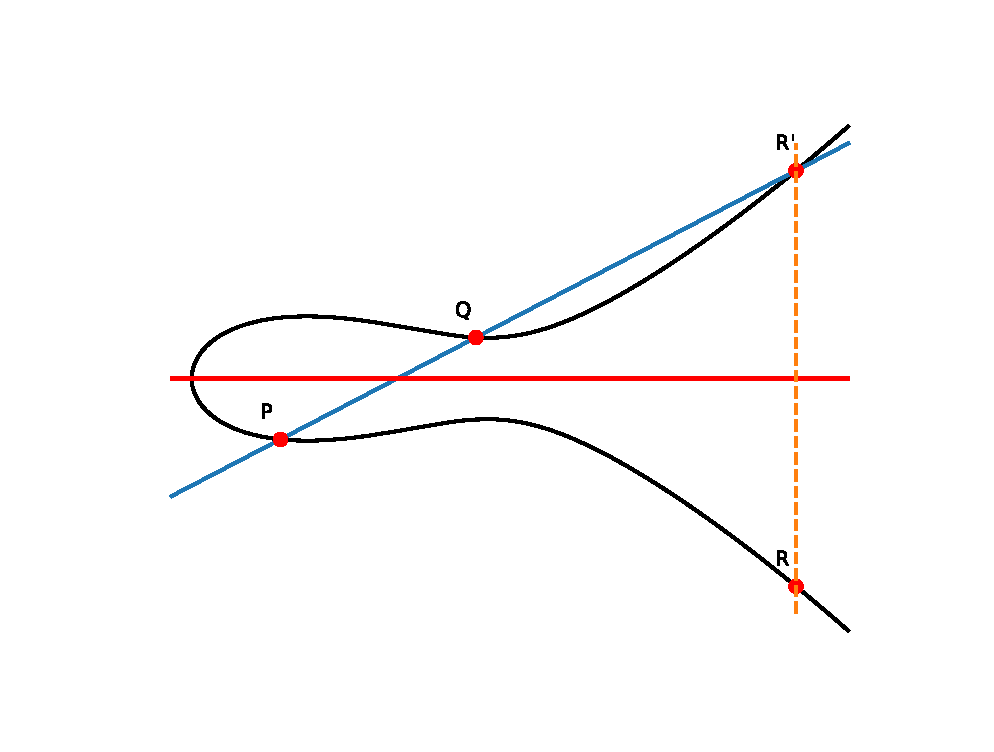
\includegraphics[width=8cm]{figures/elliptic.eps}}}%
  \qquad
  %\caption{Cálculo de $P+Q=R$}
  \subfloat[Cálculo de $2P$ y $-P$]{{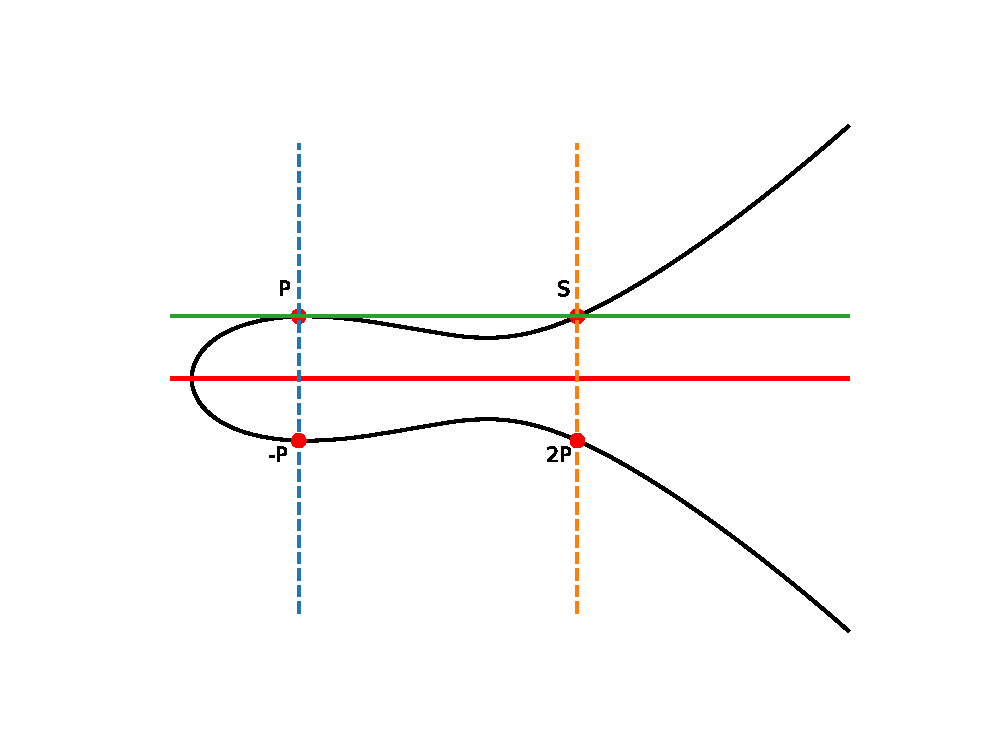
\includegraphics[width=8cm]{figures/elliptic1.eps}}}%
  %\caption{Cálculo de $2P$ y $-P$}
	\caption{Curva elíptica $y^2 = x^3 -3x + 5$}%
	\label{fig:test}%
\end{figure}
%incluir una figura
%\begin{figure}
%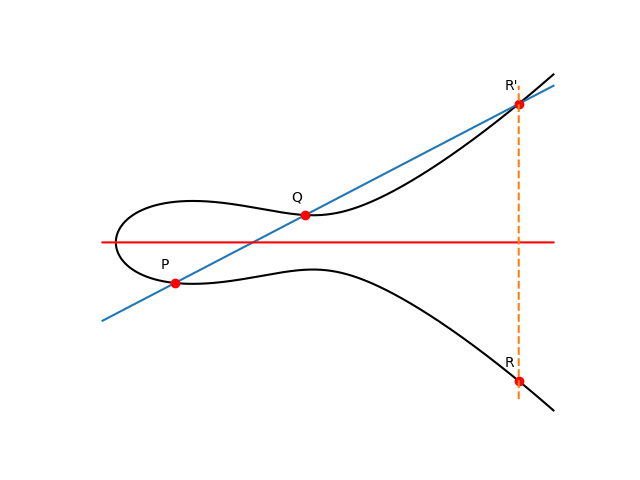
\includegraphics[height=2.9in]{figures/elliptic.png}
%\caption{Curva elíptica $y^2 = x^3 -3x + 5$}
%\end{figure}


A partir de la definición anterior de las operaciones no es difícil ver que el punto del infinito es el elemento neutro de la suma, que esta operación de suma es conmutativa y que existe el inverso de todo elemento. Sin embargo que la suma está cerrada con esta definición y que se cumple la propiedad asociativa no son resultados inmediatos. Una prueba de esto se puede consultar en \citep{group_law} y en \citep{group_law_verrill} 
%http://www.math.ku.dk/~kiming/lecture_notes/2000-2001-elliptic_curves/grouplaw.pdf 

Al cumplirse las cuatro propiedades anteriores tenemos que la suma así definida induce un grupo abeliano sobre los puntos de la curva elíptica. Sea $(G,+)$ este grupo y $n=|G|$ su orden. Sabemos que $n$ no es infinito pues la curva está definida sobre $\mathbb{K}$ un cuerpo finito, y por tanto sus puntos vendrán dados por $\{(x,y)| y^2 \equiv x^3 + ax + b  (mod  p) \}$. 
\theoremstyle{theorem}\begin{theorem}[Teorema de Cauchy]\label{cauchy} Sea G un grupo finito y q un primo. Si q divide al orden de G entonces existe un elemento de G de orden q.
\end{theorem}
Tenemos por tanto un grupo finito, donde a consecuencia del Teorema de Cauchy para grupos \ref{cauchy} podemos encontrar un elemento de orden primo $q$ (si $n = |G|$ ya es primo basta tomar $q = n$) Este elemento $g$ de $G$ genera un subgrupo cíclico ($<q>$) que será sobre el que se definan los protocolos criptográficos que veremos.


%Un subgrupo cíclico tiene orden $q$ siendo $q$ un primo tal que que $q|n$. Si $n$ es primo decimos entonces que $|G|$ es un grupo cíclico. %meter teorema de cauchy para ver la existencia de este subgrupo ciclico
%Será sobre este subgrupo cíclico sobre el que se definan los protocolos criptográficos que veremos.

\section{Funciones Hash}\label{hash}
Antes de ver el algoritmo ECDSA hay que definir el concepto de función hash y ver alguna de sus propiedades.
\theoremstyle{definition}\begin{definition}[Función Hash]\label{hash_def} Una función hash es una aplicación $\textit{H}$ entre cadenas tal que su conjunto imagen está formado por cadenas de longitud fija, siendo esta magnitud la longitud hash de la función, mientras que su preimagen está formada por cadenas de longitud arbitraria. Se escribe entonces $\textit{H}: \{0,1\}^* \rightarrow \{0,1\}^n$ si hablamos de cadenas de bits y denotamos por $n$ a la longitud hash de $\textit{H}$.\end{definition}

Aunque se hable de longitudes arbitrarias pueden existir limitaciones técnicas en cuanto a la longitud del mensaje de entrada. Considerando por ejemplo la función hash SHA-256 (SHA son las siglas de Secure Hash Algorithm) usada ampliamente en diferentes implementaciones del protocolo blockchain, que devuelve cadenas de 256 bits \citep{sha256_2}. Tenemos que esta función hash puede procesar mensajes de un máximo de $(2^{64} -1)$ bits \citep{sha256}. Es decir, que no se puede obtener el valor de hash de esta función para ninguna cadena que supere esa longitud, pero teniendo en cuenta que este valor equivale a más de 2 millones de terabytes esto no supone un verdadero problema en la práctica.

Una primera consecuencia de la definición \ref{hash_def} es que la preimagen de una función hash tiene cardinal estrictamente mayor que su imagen. Por tanto, por el principio del palomar, tendremos que si $A$ es el conjunto preimagen de cierta función hash $H$ y $B$ es su imagen para todo $b \in B$  $\exists \{a_{1},a_{2}\}$ con $a_{i} \in A$ distintos tales que $H^{-1}(b) = a_i$. Este fenómeno se llama colisión y se define en la resistencia a colisiones de una función hash como la probabilidad de encontrar un par $(a_{0},a_{1})$ con $a_{0} \not= a_{1}$ tales que se cumpla  $H(a_{0}) = H(a_{1})$. A toda función hash $H$, que usemos en el protocolo blockchain o en el algoritmo ECDSA, le pediremos que ningún algoritmo pueda encontrar una colisión para $H$ en tiempo polinómico, en este caso diremos que $H$ es resistente a colisiones. Otras dos propiedades importantes de las funciones hash serán la resistencia a preimágenes y a segundas preimágenes. La primera de estas propiedades viene a decir que debe ser \textit{díficil} dado un $b$ en el espacio de llegada encontrar un $a$ en el espacio de partida tal que $H(a) = b$. La segunda propiedad es similar a la definición de resistencia a colisiones, dado un $a_{0}$ elegido de forma aleatoria debe ser \textit{díficil} encontrar un $a_{1}$ distinto de $a_{0}$ tal que $H(a_{0}) = H(a_{1})$. Esta noción de \textit{difícil} viene dada por la imposibilidad de resolver en tiempo polinómico cualquiera de estos problemas.

La propiedad de resistencia a segundas preimágenes es  más fuerte que la resistencia a colisiones como consecuencia de la paradoja del cumpleaños. En efecto, si suponemos cadenas binarias y una longitud hash de $n$ nuestra función devolverá exactamente $2^{n}$ cadenas distintas. Dadas $l$ cadenas elegidas al azar la probabilidad de no encontrar una colisión viene dada por:
\begin{equation}
NC(n,l) = \frac{2^{n}}{2^{n}}\frac{2^{n}-1}{2^{n}}\ldots\frac{2^{n}-(l-2)}{2^{n}}\frac{2^{n}-(l-1)}{2^{n}} = \prod_{i=0}^{l-1}(1-\frac{i}{2^{n}})
\end{equation} 
Así que la probabilidad de encontrar una colisión $C(2^{n},l)$ será su complementario:
\begin{equation}
C(n,l) = 1-\prod_{i=0}^{l-1}(1-\frac{i}{2^{n}})
\end{equation}
Considerando que el cociente $i/2^{n}$ es cercano a cero, que es consecuencia de tomar $n$ suficientemente grande, y teniendo en cuenta que la expansión en Serie de Taylor de $e^{x}$ se puede truncar a partir del término cuadrático para $x \ll 1$. Tenemos que:
\begin{equation}
C(n,l) \approx 1- \prod_{i=0}^{l-1}\exp\left(\frac{-i}{2^{n}}\right) = 1- \exp\left(\sum_{i=0}^{l-1}\frac{-i}{2^{n}}\right)
\end{equation} 
Este último sumatorio se puede escribir como $-(l-1)l/2^{n+1}$ usando la fórmula de la suma de los $(l-1)$ primeros naturales. Y que para $l$ suficientemente grande se puede aproximar a $-l^{2}/2^{n+1}$.
Tomando logaritmos y despejando se tiene que:
\begin{equation}
l \approx 2^{n/2}\sqrt{-2\log(1-C(n,l))}
\end{equation}
Si se considera una probabilidad $C(n,l)$ de 0.5 entonces esa raíz cuadrada es aproximadamente 1 y por tanto $l \approx 2^{n/2}$. 

Tomando $2n = 365$ se obtiene el problema del cumpleaños: para garantizar una colisión (dos individuos que cumplan años el mismo día) con una probabilidad del $50\%$ basta con reunir 22 personas, este resultado es mucho menor que el valor que podríamos dar intuitivamente, de ahí que se le llame paradoja aunque desde el punto de vista estrictamente lógico no lo sea.

 Sin embargo, la probabilidad de encontrar una segunda preimagen comprobando solo $2^{n/2}$ cadenas es de 
$2^{n/2}/2^{n} = 1/2^{n/2}$, que para n = 64 es prácticamente cero. Para garantizar una probabilidad de al menos el 0.5 se tiene que:
\begin{equation}
k=\frac{1}{2}2^{n} = 2^{n-1} \approx 2^{n}
\end{equation}
Donde k es el número de cadenas que hay que estudiar. En este caso el coste es prácticamente el mismo que el de comprobar todas las posibles cadenas que produce nuestra función hash.

Hay que señalar que los cálculos anteriores solo son válidos bajo ciertos supuestos teóricos que en la práctica no se dan, pues ninguna función hash lleva los elementos del espacio de partida al de llegada siguiendo patrones completamente aleatorios. Una vez han sido encontradas colisiones (o se ha probado que la probabilidad de encontrarlas es \textit{alta}) la función hash deja de ser considerada segura. Un ejemplo de función hash en esta categoría es SHA-1, para la que se conocen colisiones desde 2017 \citep{sha-1}, aunque era considerada insegura desde 2005. 
La función hash que usaremos (SHA-256) es considerada segura por el momento.


%Referencias: http://web.cs.ucdavis.edu/~rogaway/papers/relates.pdf
%https://www.esat.kuleuven.be/cosic/publications/article-1532.pdf
%https://eprint.iacr.org/2004/304.pdf


%En el Bitcoin se usa en diferentes tareas la función hash SHA-256.

%trabajar esto algo mas



%una vez vista las operaciones que definen un grupo sobre la curva, especificar el algoritmo ecdsa. Luego de eso exponer el coste computacional de este algoritmo en todos los sentidos, usarlo como punto a favor del uso de curvas elipticas en lugar de logaritmos discretos u otros metodos.
\section{Algoritmo ECDSA}
%Referencia (además del libro) https://pdfs.semanticscholar.org/c06a/d6512775be1076e4abd43e3f2928729da776.pdf
%https://www.ietf.org/rfc/rfc6979.txt

Ahora podemos especificar el algoritmo ECDSA (Elliptic Curve Digital Signature Algorithm)\citep{elliptic_cripto}, tanto el usado para la firma de mensajes como el correspondiente algoritmo de verificación. Este algoritmo se basa en la dificultad computacional de resolver el problema del logaritmo discreto para curvas elípticas (ECDLP).

\theoremstyle{definition}\begin{definition}[Problema del logaritmo discreto para curvas elípticas]\label{ecdlp} Sea $E(\mathbb{K})$ una curva elíptica sobre un cuerpo $\mathbb{K}$. Sea $P \in E(\mathbb{K})$ y $Q \in <P>$. Encontrar $k$ tal que $Q= kP$. \end{definition}

La definición anterior tiene sentido pues como se vio en \ref{curvas_grupo} los puntos de una curva elíptica definida sobre un cuerpo finito forman un grupo. En este caso $<P>$ es el subgrupo ciclico generado por el elemento $P$ de la curva. 

No se conoce algoritmo que resuelva este problema en tiempo subexponencial \citep{discrete_log}. Sin embargo, aunque aquí no serán especificados se necesitan algoritmos apropiados para crear y representar el cuerpo finito $\mathbb{F}_{p}$ de forma que se garantice la intratabilidad de este problema.
%El orden de una curva elíptica $E$ sobre un cuerpo finito $\mathbb{F}_{p}$ (número de puntos) es importante para garantizar la seguridad de este algoritmo.

Antes de poder firmar un mensaje hay que generar las claves públicas y privada.
Sea $P = (x_{1},y_{1})$ un punto de la curva elíptica $E(\mathbb{F}_{p})$ que genera un subgrupo cíclico $<P>$ de orden primo $n$. El par $(d,Q)$ de claves privada y pública se genera usando el algoritmo \ref{alg:claves}. La elección aleatoria de $d$ es muy importante, en otro caso se pueden tener problemas de seguridad (un ejemplo de esto fue el hackeo del software de la PS3 de Sony por el grupo fail0verflow en 2010).
\begin{algorithm}
\caption{Generación de claves}\label{alg:claves}
\begin{algorithmic}[1]

\State Se elige $d \in [1, n-1]$ de forma aleatoria

\State Se calcula $Q=dP$

\State  $Q$ es la clave pública y $d$ la clave privada.
\end{algorithmic}
\end{algorithm}


Una vez se ha generado la clave privada y utilizando una función hash $H$ que devuelva cadenas de longitud menor o igual que $n$ se pueden firmar mensajes usando el algoritmo \ref{alg:firmar}
\begin{algorithm}[H]
\caption{Generación de firma}\label{alg:firmar}
\begin{algorithmic}[1]
\State Se elige $k \in [1, n-1]$ de forma aleatoria
\State Se calcula $z_{1} = kx_{1}$ 
\State Se calcula  $r = z_{1} (mod  n)$ si $r = 0$ paso 1.
\State Se calcula $e = H(m)$
\State Se calcula $s = k^{-1}(e + dr) (mod n)$ si $s = 0$ paso 1. \Comment{$k^{-1}$ es el inverso de k en el grupo $<P>$}
\State Se devuelve $(r,s)$
\end{algorithmic}
\end{algorithm}

Ahora, quien recibe un mensaje $m$ con la firma $(r,s)$ puede verificar su procedencia (suponiendo que ha recibido antes la clave pública $Q$) mediante el algoritmo \ref{alg:verificar}

\begin{algorithm}
\caption{Validación de firma}\label{alg:verificar}
\begin{algorithmic}[1]
\State Verificar que $r,s \in [1, n-1]$, en otro caso \textbf{se rechaza la firma}
\State Se calcula $e = H(m)$
\State Se calcula $w = s^{-1} (mod n)$
\State Se calcula $u_{1} = ew (mod n)$, $u_{2} = rw (mod n)$
\State Se calcula $X = u_{1}P + u_{2}Q$, si $X=\infty$ \textbf{se rechaza la firma} \Comment{$X \in E(\mathbb{F}_{p})$}
\State Sea $X = (x_{1},y_{1})$, se calcula $v = x_{1} (mod n)$
\State Si $v = r$ \textbf{se acepta la firma}, en otro caso \textbf{se rechaza la firma}
\end{algorithmic}
\end{algorithm}

La importancia de la resistencia a colisiones en la función hash $H$ queda explicada con los algoritmos anteriores.
La existencia de colisones conocidas (o facilmente calculables) hace que ya no sea posible garantizar la validez de una firma. Un atacante podría usar un mensaje firmado, buscar alguna modificacion de este mensaje que combinada con la firma devuelva el mismo valor hash que en el original. Ahora quien verifique este mensaje falso seria incapaz de distinguirlo del original.

%(Poner imagen de https://shattered.it/ como ejemplo de colision)

%mirar https://webusers.imj-prg.fr/~ricardo.perez-marco/blockchain/BitcoinP7.pdf en los referente a hash
\cleardoublepage

\chapter{Especificación del protocolo blockchain}
\label{cap3}
Una vez se han visto las dos nociones criptográficas fundamentales en las que se fundamenta el blockchain (algoritmo ECDSA y funciones Hash) es posible explicar tanto el funcionamiento de este protocolo como justificar su corrección. 
Aunque las ideas fundamentales que serán expuestas están basadas en el artículo original del Bitcoin \citep{bitcoin} en los puntos en los que existan divergencias entre distintas implementaciones del protocolo se intentarán señalar las diferentes alternativas. Siendo esta una tecnología que se ha desarrollado más con la práctica a través de diversas implementaciones que con trabajos teóricos resulta complicado abarcar en un solo trabajo todas sus variantes.

\section{Objetivos del Blockchain}\label{objetivos}
El Bitcoin surgió con el objetivo de por un lado eliminar la necesidad  de una entidad de confianza que actúe de intermediario en las transacciones económicas digitales y por otro lado de resolver el problema derivado de la ausencia de este ente. En un intercambio basado en artículos físicos a los que se le asigna cierto valor (el papel moneda por ejemplo) los únicos problemas de los que las partes deben preocuparse son aquellos derivados de la estafa o la falsificación. Cuando estas transacciones se realizan sin intervenir medios físicos no se puede garantizar que la parte encargada de entregarle la retribución monetaria a la otra posea los medios económicos que dice tener. Más aún, alguien aún disponiendo de la capacidad de realizar cierta transacción puede enviarle a diferentes individuos cantidades que por separado no superen sus fondos, pero que en conjunto sí lo hagan, este es el llamado problema del doble gasto. Los intermediarios cumplen entonces la función de evitar que esto ocurre al llevar un registro actualizado de las transacciones de cada cliente y por tanto de los fondos de los que dispone.

Pero, ¿qué sentido tiene entonces eliminar el intermediario si con ello solo generamos problemas que debemos resolver? Un sistema descentralizado tolera mucho mejor las particiones que uno centralizado: basta aislar al servidor para dejar inoperativa toda la red. Además, desde el punto de vista de la seguridad cualquier ataque con éxito al servidor supone a su vez la caída de todo el sistema. Incluso suponiendo que se dispone de un intermediario seguro y distribuido en diferentes nodos de forma que la caída de alguno de ellos no suponga mayor problema para la red, la pregunta que debemos hacernos es cuanto podemos llegar a confiar en esta entidad. En la medida en que controla nuestro dinero puede llegar a actuar de forma más o menos arbitraria con él ya sea por interés propio o al servicio de algún poder externo. Ejemplos en la vida real hay muchos.

El objetivo será por tanto proporcionar un protocolo seguro, que aún estando completamente descentralizado pueda resolver en particular el problema del doble gasto y en general problemas de consenso de otra clase. Por tanto, la corrección de este protocolo vendrá dada por la comprobación de que justamente se han solucionado estas cuestiones.
%Como se mencionó en la introducción, el blockchain consiste en esencia en un registro distribuido e inmutable

\section{Configuración de la red}
El protocolo blockchain se define e implementa sobre una red basada en la arquitectura peer-to-peer (red entre pares). El término peer-to-peer (en lo adelante P2P) viene a decir que al contrario que en un sistema cliente/servidor aquí todos los nodos realizan potencialmente las mismas funciones. Este punto puede no ser del todo cierto en determinadas implementaciones como por ejemplo en Blockchain de consorcio o privados, pero en estos casos es el protocolo elegido y no la estructura de la red quien restringe las funciones de algunos nodos. Estas restricciones no limitan en ningún caso la capacidad de enviar o recibir información directamente entre los participantes, sino que está controlada que clase de información determinados nodos pueden enviar y como los demás interpretan estos mensajes. El Bitcoin es el ejemplo más importante de red blockchain donde no hay ninguna clase de jerarquía 

Aunque todos los nodos teóricamente puedan realizar las mismas funciones en la práctica suelen elegir que tareas realizar y cuales ignorar. Así, algunas máquinas pueden dedicarse a ejecutar las labores más complejas del algoritmo de consenso (más adelante veremos en que consiste este algoritmo), otras  almacenan parte (o la totalidad) de la cadena de bloque, mientras que otros nodos ejecutan tareas de verificación. Existen otras especializaciones (o combinaciones de especializaciones) que pueden variar entre diferentes implementaciones del blockchain.

%La información transmitida desde un punto en una red P2P debe alcanzar a casi todos los nodos, extenderse algo más aquí.
Un problema importante en las redes es p2p es como los participantes se encuentran unos con otros para establecer una conexión. Los nodos mantienen un registro privado de las direcciones ip con las que se han comunicado, y pueden compartir este registro con otros miembros que lo soliciten, esta sería la forma estándar de ampliar la agenda de contactos. La primera vez que un nodo se une a la red dispone de una lista de direcciones ip prefijada, en ciertos protocolos blockchain que han alcanzado un número de participantes considerable existe también la posibilidad de conectarse a varias DNS Seeds donde recibe una lista generada aleatoriamente de otros nodos que han estado activos en la red en un rango de tiempo determinado. Este punto, dado que es el único en el que existe algo de centralización, entraña ciertos riesgos, pues alguno de estos DNS Seed puede caer bajo el control de una entidad maliciosa que le proporcione a los nuevos participantes solo direcciones ip de nodos bajo su control, de esta forma se podría crear una red independiente de la principal donde existe una cadena de bloques generada de forma arbitraria. Por ello se mantiene cierto control de forma pública y abierta sobre estas DNS Seed y se puede igualmente usar direcciones ip  recibidas a través de cualquier otra vía.


\section{Cadena de bloques}\label{bloques}
El componente fundamental del blockchain es la estructura de datos donde se almacena toda la información que los nodos que participan en el protocolo han acordado que es válida. En las criptomonedas este registro cumple la función de libro de cuentas, sin embargo, se pueden guardar todo tipo de datos.

Cada uno de los bloques que conforman esta cadena además de la propia información que pueda contener mantiene una referencia al bloque anterior. La excepción a esto es el bloque inicial, que se genera de forma diferente al resto.
Esta estructura enlazada no es suficiente para garantizar la integridad de la cadena de bloques, pues un adversario podría modificar la información almacenada en un bloque dejando intacta la referencia al bloque anterior. Aquí es donde se utilizan por primera vez las funciones hash definidas en \ref{hash}: además de la información almacenada y la referencia al bloque anterior guardaremos también el resultado de aplicar cierta función hash al conjunto de los datos del bloque (incluido quien es el bloque anterior). Si la función elegida es resistente frente a segundas preimágenes se puede verificar que  el bloque es correcto simplemente aplicándole la función Hash a sus datos y comparando con la almacenada. Y la referencia al bloque anterior en lugar de ser únicamente un índice incluirá también el valor hash de ese bloque.

Sin embargo, aún con este añadido seguimos sin tener garantizado que un adversario pueda hacer modificaciones en la cadena. Es cierto que ahora para hacer cambios en un único bloque tendría que generar nuevamente toda la cadena a partir de ese bloque, pero el coste de operar con funciones hash es lineal, así que es factible hacer estas modificaciones en un tiempo razonable. Además de la referencia al bloque anterior y la información del bloque actual en los datos que sobre los que se aplica la función hash se incluirá un valor generado de forma aleatoria, así se garantiza que la cadena hash resultante tenga ciertas propiedades definidas en el protocolo. Por ejemplo, en el Bitcoin a la cadena hash se le pide que comience por cierto número de ceros. El cálculo de este valor aleatorio, denominado nonce (number used once), es la tarea principal del algoritmo de prueba de trabajo que se verá en el siguiente apartado.

Otra información que se incluye en los bloques, asociada con la función hash, es una marca temporal (timestamp) del momento en que fue creado el bloque. De esta forma se puede probar que la información existía cuando se calculó el valor hash. Mantener un registro temporal también servirá en el algoritmo de consenso para rechazar directamente aquellos bloques con marcas de tiempo superiores al momento actual.

Por último, y con el objetivo de reducir el uso de espacio, el conjunto de operaciones almacenadas en un bloque no se guardan explícitamente. En su lugar se almacena la raíz del arbol Merkle resultante. En la siguiente sección esta estructura de datos será analizada.

Lo anterior se puede considerar más o menos estándar en todas las implementaciones del blockchain, pero se pueden incluir otros elementos dentro de cada bloque.
\begin{figure}[H]
%\centering
  \subfloat[Diagrama Blockchain (Fuente \url{http://www.doc.ic.ac.uk/~ma7614/topics_website/tech.html}
)]%
  {{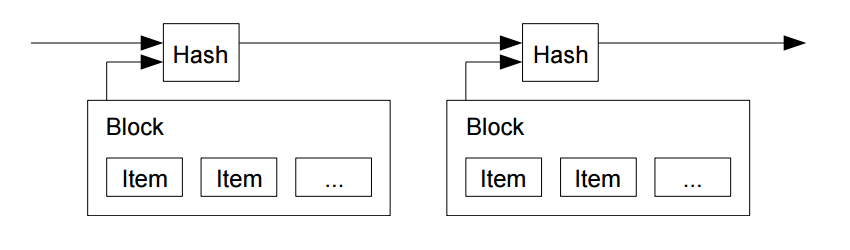
\includegraphics[width=12cm]{figures/blockchain_diagram.png}}}%
  \qquad

	\label{fig:blockchain}%
\end{figure}

\section{Árboles Merkle}\label{merkle}
Los arboles Merkle, patentados en 1979 por Ralph Merkle han sido usados activamente en la verificacion de bases de datos (cita: https://coincentral.com/merkle-tree-hashing-blockchain/)
En el caso del Blockchain para cada transaccion se calcula su valor hash, combinando estos resultados en pares se reduce a la mitad el numero de valores que hay que almacenar. Repitiendo este proceso, ahora para los valores resultantes se llega a un valor hash final, llamado raiz hash, que se ha calculado de forma deterministica a partir de los valores originales (transacciones).

Por ejemplo, si se desean guardar las transacciones A,B,C,D en cierto nodo calculamos en primer lugar, H(A), H(B), H(C), H(D) donde H es la funcion hash que estemos utilizando. Posteriormente se calcula H((H(A),H(B) y H(H(C),H(D)), por ultimo queda aplicarle la funcion H a estos dos valores, y se tiene entonces la raiz Merkle que se incluira en el bloque.

Por las propiedades de las funciones hash vistas antes, se garantiza la integridad de las transacciones almacenadas, pues cualquier ligera modificacion en las mismas produciria cambios en la raiz Merkle resultante y por tanto ese bloque se rechazaria. Ademas, la propia estructura de los arboles Merkle nos permite encontrar que transaccion ha cambiado, pues basta descender desde la raiz comparando cada uno de los valores hash almacenados hasta encontrar la transaccion, que viene a ser una hoja del arbol, que ha sido modificada.

\begin{figure}[H]
\centering
  \subfloat[Diagrama Árbol Merkle (Fuente \url{https://www.researchgate.net/publication/324385574_Towards_Decentralized_Accountability_and_Self-sovereignty_in_Healthcare_Systems}]{{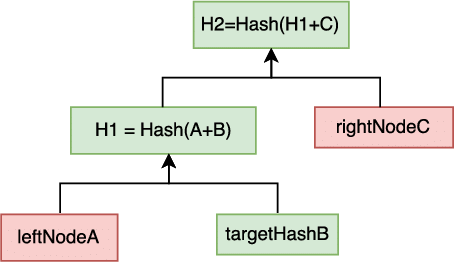
\includegraphics[width=12cm]{figures/merkle_tree.png}}}%
  \qquad

	\label{fig:merkle}%
\end{figure}


\section{Algoritmo de prueba de trabajo}\label{chap3:pow}
La estructura en cadena de bloques enlazados usando funciones hash no resuelve por si sola el problema del doble gasto visto en \ref{objetivos}, para eso hay que establecer un algoritmo que permita a los participantes decidir que información se puede incluir en la cadena de bloques, validando de esta forma las transacciones correctas. En el Bitcoin se estableció como tal sistema el algoritmo de prueba de trabajo (Proof of Work), en posteriores implementaciones del blockchain, salvo ciertas modificaciones se ha mantenido en general este mismo algoritmo. La idea de la prueba de trabajo se originó para resolver el problema del uso abusivo de ciertos recursos como el correo electrónico mediante el envío masivo de mensajes de spam. Hashcash \citep{hashcash}, una de las primeras implementaciones de un mecanismo para solucionar este problema, se basaba en usar una función de coste para generar una ficha que permitiría disponer de cierto recurso. Esta ficha probaba que el usuario había invertido determinado tiempo de procesamiento en resolver el problema planteado por la función de coste y de esta forma el uso del recurso en cuestión estaba condicionado por la inversión en procesamiento del usuario. Con el Bitcoin este planteamiento basado en un sistema cliente-servidor fue extendido a un contexto descentralizado.

El resultado de ejecutar la función de coste (ficha) debe poder ser verificado fácilmente por cualquiera, mientras que el cálculo de esta función debe ser una tarea moderadamente complicada. La funciones hash cumplen estos requisitos y son usadas como función de coste. Un participante que quiera validar un bloque, es decir, que quiera afirmar que cierto conjunto de transacciones o datos son válidos y que por tanto se pueden añadir al registro toma el bloque tal y como se definió en \ref{bloques} le añade cierto valor en bits cuya posible longitud y posición dentro del bloque están determinados en el protocolo y analiza el resultado de aplicarle cierta función hash acordada. Si este resultado cumple ciertos requisitos (por ejemplo la cadena hash devuelta empieza por $n 0's$) entonces se dice que se ha resuelto el problema del algoritmo de prueba de trabajo (llamado puzzle en algunas fuentes) y se comparte con los demás nodos este resultado. Puede encontrarse también en ciertos artículos y especificaciones de criptomonedas que el puzzle que se debe resolver para validar cierto bloque consiste en encontrar una cadena hash menor que cierta longitud. Esto no es más que buscar cadenas hash que comiencen con ciertos número de ceros y considerarlas como de tipo numérico donde esos ceros desaparecen dejando una cadena $n$ posiciones más corta que la longitud hash de la función del algoritmo. 

En el algoritmo \ref{alg:pow} se presenta una posible especificación (muy simplificada) del método de prueba de trabajo para calcular un nonce  asociado a cierto bloque. En esta especificación se supone que quien la ejecuta ha verificado antes que todas los datos que se pretenden incluir en la cadena son correctos. Este algoritmo tal y como está planteado puede no terminar, pues es posible que no exista ningún nonce de longitud menor o igual que $m$ que resuelva el puzzle. En la práctica si el bloque $b$ está formado por cadenas de la forma $b = s+p+k+t_{1}+ \ldots + t_{q}$ donde $s$ es el timestamp, $p$ la referencia al valor hash del bloque anterior, $k$ es la clave pública del nodo que está calculando el nonce y $t_{i}$ el conjunto de datos que almacena el bloque, se suele proceder reordenando los $t_{i}$ a la vez que se modifica el nonce y comprobando el resultado de estas combinaciones. También se suelen hacer pequeñas modificaciones en el timestamp $s$, pues entre la hora marcada por el bloque anterior y lo que se tarda en generar el siguiente bloque hay un rango de tiempo en el que moverse. Este proceso es lo que se conoce en las criptomonedas como minado. Las implementaciones de este algoritmo deben incluir, una condición de parada extra, pues no tiene sentido seguir operando si alguien ya ha resuelto el puzzle, así, se debe mantener un proceso que en caso de recibir información sobre la resolución (correcta) del problema de prueba de trabajo para el bloque en el que se está trabajando detenga el algoritmo. 

\begin{algorithm}
\caption{Prueba de trabajo (Cálculo)}\label{alg:pow}
\begin{algorithmic}[1]
\Require \Statex $H$ función hash del protocolo de longitud de cadena $k$.\Statex $l$ < $k$ longitud (dificultad) del puzzle.\Statex $m$ longitud máxima del nonce.\Statex $b$ bloque que se quiere validar.
\State Generar \textit{nonce} de forma aleatoria tal que $|nonce| \leq m$ \label{alg:pow:step1}
\If{$|H(nonce+b)| \leq l$} \Return $(nonce, b)$
\Else  Volver a  \ref{alg:pow:step1}
\EndIf
\end{algorithmic}
\end{algorithm}

Se incluye también el algoritmo de verificación que deben utilizar los nodos para comprobar el par $(nonce, b)$. Si acepta el bloque la forma de comunicarlo al resto de la red es incluir ese bloque en la cadena y empezar a trabajar en uno nuevo que lo tenga como predecesor. Puede ocurrir que diferentes nodos acepten distintos bloques en determinado punto, esto se denomina bifurcación y se trata en la siguiente sección.
\begin{algorithm}
\caption{Verificación de la prueba de trabajo}\label{alg:pow_check}
\begin{algorithmic}[1]
\Require \Statex $H$ función hash del protocolo de longitud de cadena $k$.\Statex $l$ < $k$ longitud (dificultad) del puzzle.\Statex $m$ longitud máxima del nonce. \Statex $(nonce, b)$
\State Se comprueba que $b$ está formado por datos válidos (bloque previo, timestamp y transacciones). Si falla cualquiera de estas comprobaciones \textbf{rechazar}
\If{$|H(nonce+b)| \leq l$} \Return \textbf{aceptar el bloque}
\Else  \textbf{ rechazar}
\EndIf
\end{algorithmic}
\end{algorithm}

\begin{figure}[H]
%\centering
  \subfloat[Proceso pow (cambiar esta imagen (rehacer en python)]{{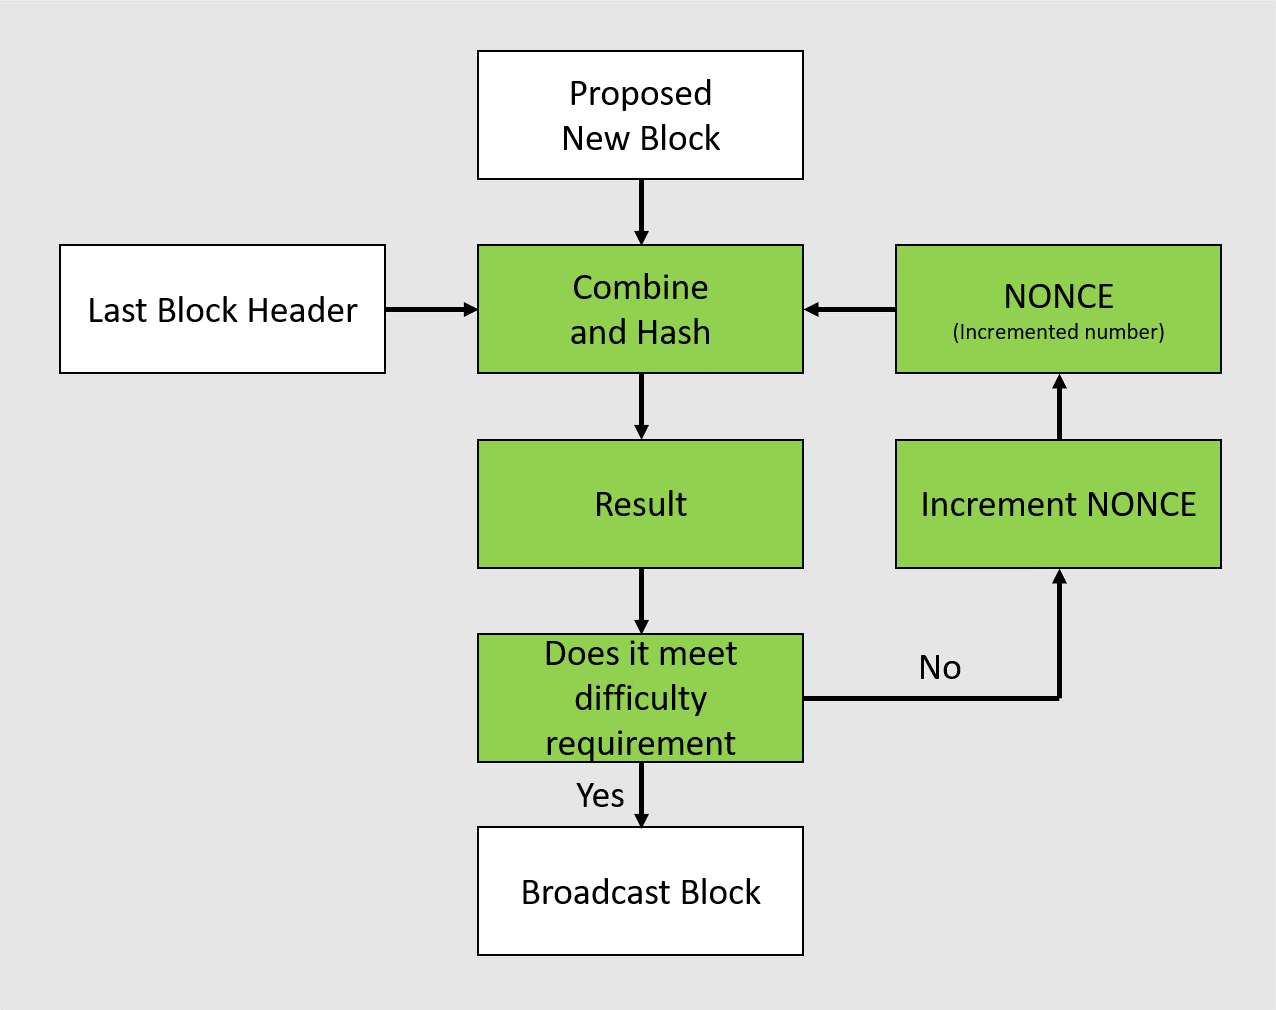
\includegraphics[width=12cm]{figures/process_to_modify.png}}}%
  \qquad
  %\caption{Cálculo de $P+Q=R$}
  %\caption{Cálculo de $2P$ y $-P$}
	\label{fig:flux}%
\end{figure}

La dificultad del puzzle, es decir, la condición que se le pide al valor hash del bloque para ser aceptado, en general no se mantiene fija. Cada determinado número de bloques (fijado en el protocolo) se vuelve a calcular este valor usando cierta función dependiente de la dificultad actual del puzzle. De esta forma según crece la cadena es necesario invertir más recursos en añadir un nuevo bloque.
% Crear un tkinter en python donde se pueden hacer pruebas e incluirlo en el apéndice.
\section{Escalabilidad del blockchain}

Explicar como ha medida que crece la red esta se fortalece, pero poner también algo referente a como aumenta la complejidad del algoritmo para validar un nonce en el blockchain, quizás poner también algun gráfico de como aumenta este coste.


\section{Resistencia a ASIC}
%hablar un poco de la asic
Con el aumento en la popularidad del Bitcoin, y de otras criptomonedas similares, se generalizó el uso de hardware dedicado exclusivamente al minado, es decir, a resolver el problema planteado por el algoritmo de prueba de trabajo visto en \ref{chap3:pow} El desarrollo de esta clase de hardware ha hecho que resulte prácticamente imposible utilizar ordenadores de uso doméstico durante el proceso de minado, lo que llevado a multiples usuarios a dejar de participar en el proceso de creación y validación de la cadena de bloques, delegando en terceros este proceso. Esta delegación de la confianza en una tercera entidad va en contra de los principios fundamentales del Blockchain. Se tienen entonces dos problemas fundamentales: por un lado el desarrollo de hardware especifico que en la práctica excluye a una parte de los usuarios de participar en el algoritmo de prueba de trabajo, por otro lado, este algoritmo hace posible delegar en otra entidad (los llamados mineros) el proceso de creación de nuevos bloques en la cadena, haciendo que parte de los usuarios no participen activamente en el proceso.
\begin{figure}[H]
%\centering
  \subfloat[Ejemplo de dispositivo ASIC (Fuente: amazon.com)]{{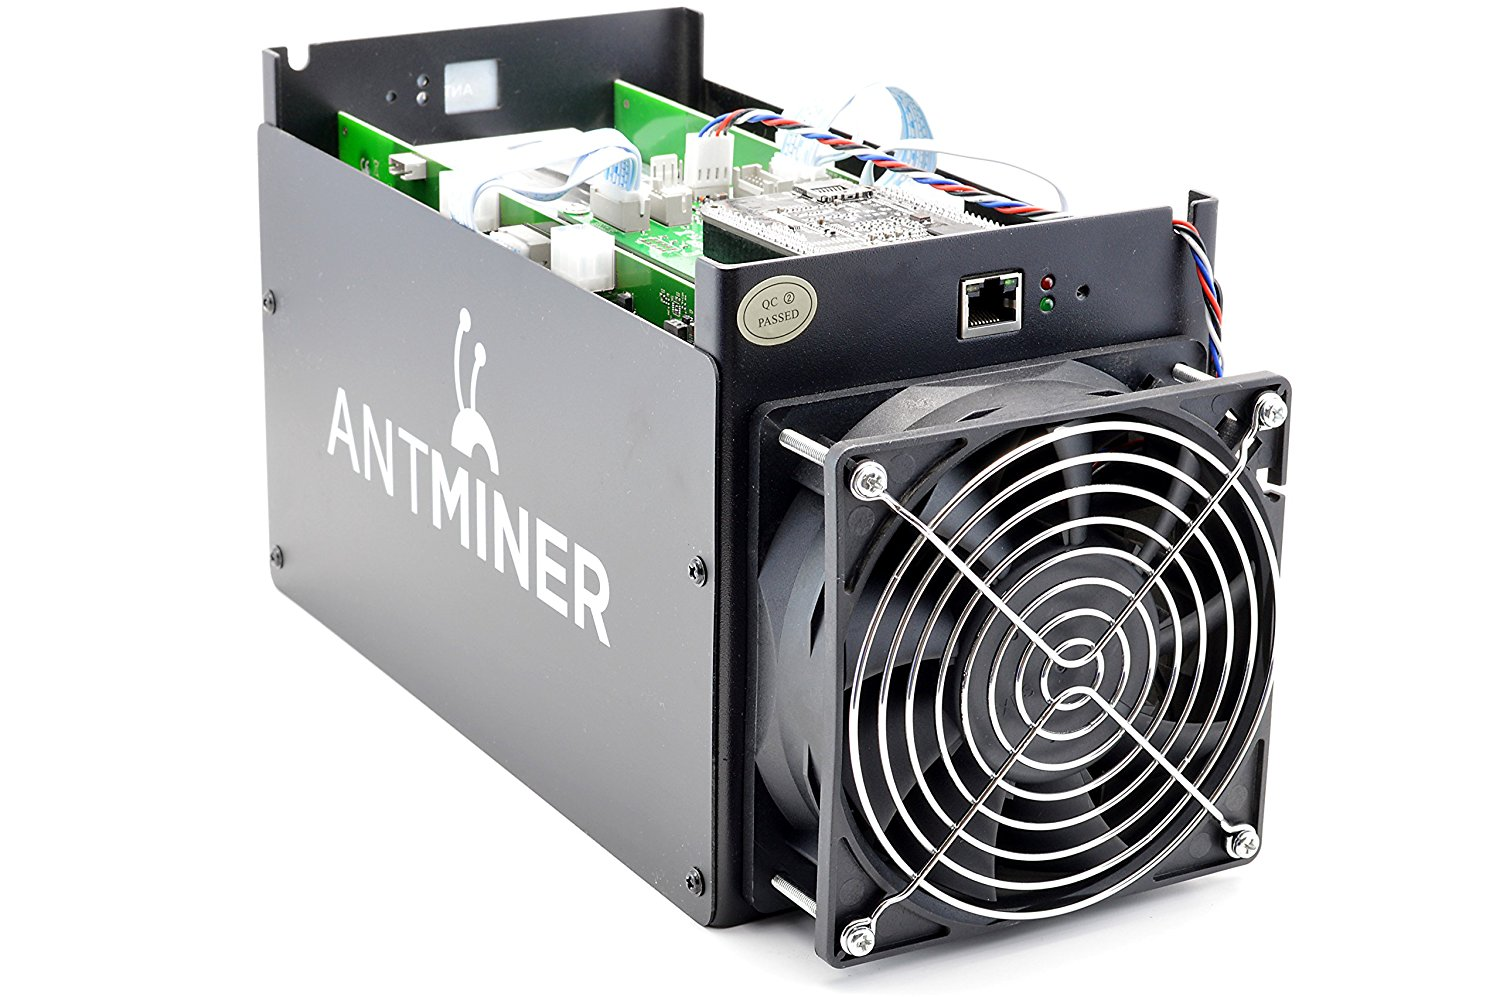
\includegraphics[width=12cm]{figures/asic.jpg}}}%
  \qquad
  %\caption{Cálculo de $P+Q=R$}
  %\caption{Cálculo de $2P$ y $-P$}
	\label{fig:test}%
\end{figure}
Estos son los motivos del desarrollo de algoritmos resistentes al minado mediante ASIC’S y que a su vez intentan minimizar la creación de nodos dedicados exclusivamente a este proceso, como las llamadas mining pools del Bitcoin. Uno de los principales algoritmos cuyo objetivo es combatir estos problemas es Hashimoto (http://diyhpl.us/~bryan/papers2/bitcoin/meh/hashimoto.pdf). Se trata este de un algoritmo basado en E/S, otros algoritmos creados para este fin se basaban por ejemplo en el mayor uso de memoria, pero para estos con el tiempo ha ido surgiendo hardware especifico.

 La idea base detrás de Hashimoto no es hacer un algoritmo que sea resistente a ASIC, sino un algoritmo que funcione de forma óptima en ordenadores de uso doméstico, basado en el hecho que los límites de lectura-escritura son un problema estudiado durante años en el campo de la computación y es poco probable que el minado de monedas produzca avances significativos en esta área, y en caso de producirlos su trascendencia seria tal que impactarían en la industria del hardware en general.
Tanto en el caso de del algoritmo Hashimoto, como en el algoritmo de prueba de trabajo visto antes (cita) un valor hash correcto es aquel que cumple que su longitud es menor que cierto valor dado, es decir, que el valor hash empieza por n-ceros.

Este valor hash resulta de aplicar cierta función hash (sha-256 en el caso del Bitcoin) al bloque anterior, raíz merkle y cierto nonce. La raíz Merkle como se vio en \label{merkle} está basada en las transacciones del bloque que se quiere incluir. 


Hasta este punto Hashimoto y el método de prueba de trabajo visto antes coinciden. En lugar de detenerse en el valor hash obtenido hasta este momento en Hashimoto se realiza un segundo procesado de los datos. El conjunto de transacciones almacenados en la cadena de bloques puede considerarse ordenado. Por ejemplo la transacción número 10 del bloque 11 , podría tener el índice numero 560. Lo que hace ahora Hashimoto es acceder a diferentes puntos de la cadena, basandose en el orden anterior y en el valor hash calculado originalmente. El numero de transacciones de la cadena a las que accede es un numero fijado por el algoritmo. Se tiene entonces un conjunto de operaciones extraidas de diferentes puntos de la cadena de bloques para las que se calcula su valor hash.


El resultado (solucion del algoritmo de prueba de trabajo) sera el nonce que resuelva el algoritmo de prueba de trabajo para esta combinacion de valores. Asi, se tiene que Hashimoto depende de acceder a casi la totalidad de la cadena de bloques. Para cadenas de bloques pequenas esto no es un problema, pues pueden tenerse en memoria. Pero cuando estas cadenas deben mantenerse en disco por su longitud, es entonces cuando se aprecia el efecto de los tiempos de acceso de E/S. Ademas, se obliga a los participantes a tener una copia completa de la cadena de bloques, de otra forma dependen de la respuesta de otros nodos que almacenen el bloque para el cual quieren consultar cierta transaccion. 

El algoritmo Etash, usado actualmente en la criptomoneda Ethereum esta basado en Hashimoto. Este algoritmo busca (cita: https://github.com/ethereum/wiki/wiki/Ethash-Design-Rationale) 4 objetivos fundamentales:
\begin{itemize}
    \item \textit{Saturar E/S} Debe forzarse el uso de casi toda la memoria RAM, basandose en el hecho que el tamano de RAM en los ordenadores de uso domestico, particularmente en las GPU's se encuentra por encima de los disponibles en dispositivos ASIC
    \item \textit{Funcionamiento optimo en GPU's} Se busca que el minado mediante GPU's sea lo mas facil posible, dado que optimizar este minado en CPU's 
    \item \textit{Facilmente verificable} Cualquier participante debe ser capaz de verificar en un tiempo razonable una nuevo bloque.
    \item \textit{Favorecer a los clientes que almacenan la totalidad de la cadena} Aquellos que dedican espacio de almacenamiento propio para guardar la cadena de bloques tendran tiempos de acceso menores a los diferentes bloques y por tanto cierta ventaja.
\end{itemize}

\section{Uso de GPUs} %cambiar a hardware o algo asi
El algoritmo de prueba de trabajo visto en \ref{chap3:pow} se puede implementar usando computación paralela. De hecho esta es en general la forma óptima\footnote{\url{https://en.bitcoin.it/wiki/Why_a_GPU_mines_faster_than_a_CPU}} de implementarlo, pues cada procesador se encarga por separado de analizar cierto grupo de posibles valores para encontrar la solución del puzzle. Las unidades de procesamiento grafico o GPU por sus siglas en ingles (Graphic Processing Unit) estan dotadas de un mayor numero de unidades aritmetico-logicas asi como de hilos de proceso, por este motivo resultan mucho mas efectivas en comparacion con las CPU para realizar el minado. En los supuestos en los que se han tomado medidas en el algoritmo de consenso para evitar el uso de harware especifico de minado se convierten en la opcion mas efectiva.


Esto, por otro lado contribuyó el aumento del precio de las tarjetas gráficas\footnote{https://cointelegraph.com/news/report-analyst-finds-nvidia-earned-135-billion-more-in-total-crypto-revenue-than-stated (buscar otra)}
Una alternativa a las GPUs es el uso de circuitos integrados de aplicación específica o ASIC por sus siglas en inglés (application-specific integrated circuit) diseñados para minar de forma óptima ciertas criptomonedas. Existen sin embargo variantes del algoritmo de prueba de trabajo que introducen cierta resistencia tanto al minado a través de ASIC como mediante GPU \footnote{https://coincentral.com/asic-gpu-cpu-mining/}

\section{Bifurcaciones}\label{cap3:bifurcaciones}
Cuando se envían por la red varias versiones correctas del siguiente bloque los nodos pueden recibirlas en diferente orden. Por protocolo incluirán la primera que han recibido, así que puede ocurrir que la cadena de bloques deje de ser única. Para resolver este problema cada nodo almacena las otras versiones del último bloque que ha recibido, aunque solo considere como buena una de ellas. Con el cálculo de un nuevo bloque alguna versión se hará mas extensa que las otras (tendrá un bloque nuevo) y en este caso todos los nodos que estuvieran en una rama distinta de la cadena cambiarán a la versión más larga.

Hay que señalar que el término bifurcación (fork) es usado también en la literatura sobre el blockchain para designar el proceso en el que se produce una modificación del protocolo acordada (o no) por los participantes. Cuando esto ocurre quienes siguen trabajando con una versión anterior dejan de reconocer los mensajes que se producen la nueva. Los que participan en este cambio pueden o bien dejar de reconocer también al protocolo antiguo y se dice entonces que estamos ante una bifurcación dura (hard fork) o seguir aceptando estos mensajes y se dice entonces que se ha producido una bifurcación suave (soft fork). Con esto se busca corregir errores en el código, prevenir ataques a la cadena de bloque o simplemente introducir mejoras.

La resistencia a ASIC introducida en la criptomoneda ethereum, así como sucesivas transformaciones 
%poner ejemplo del bitcoin y del ethereum, hablar de como con esto se previene la creacion de hardware de minado especifico para determinado protocolo, hablar también de bifurcaciones accidentales
%\section{Árboles Merkle}

%definir y explicar como se usan
\section{Alternativas a la prueba de trabajo}
El método de prueba de trabajo explicado en \ref{chap3:pow} al estar basado en la realización de un gran número de operaciones, ya sea en CPU, GPU o ASIC tiene ciertos inconvenientes. Por un lado, entidades con el poder suficiente para controlar un gran número de máquinas pueden intentar alterar el protocolo de consenso en la red. Como vimos esto se intenta solucionar, al menos parcialmente, al introducir medidas contra el minado usando hardware específico, permitiendo de esta forma que los usuarios domésticos participen en igualdad de condiciones. Pero nada impide que ciertas entidades utilicen gran numero de CPU's o GPU's para intentar hacer modificaciones en la cadena de bloques.
En general la filosofía del blockchain supone que alguien que tiene interés en participar en el protocolo y lo demuestra invirtiendo su tiempo de procesamiento estará también interesado en que el consenso se mantenga y por tanto no validará operaciones falsas. Igualmente, se pueden utilizar las bifurcaciones explicadas en \ref{cap3:bifurcaciones} para modificar el protocolo si es necesario contrarrestar algún tipo de hardware específico diseñado para hacer más efectivo el proceso de minado.
 %(en el enlace \url{goo.gl/xn4D5s} se puede ver un ejemplo de esto).url https://ethereumworldnews.com/ethereum-hard-fork-proposed-in-response-to-new-asic-miners/

Otra de las consecuencias negativas del protocolo de prueba de trabajo es de índole ecológica. El coste computacional de una red grande, como la de las criptomonedas Bitcoin y Ethereum por ejemplo, se refleja en un gasto energético extraordinario. Hay que tener en cuenta que en el proceso de validar un conjunto de operaciones solo se tiene en cuenta el resultado del primero que resuelve el puzzle, y por tanto el trabajo de todos los que han estado trabajando en ese mismo bloque ha sido en vano. Se estima que la red del Bitcoin a finales de 2017 ya gastaba más energía eléctrica que 159 países \citep{electricidad}. Teniendo en cuenta que las principales fuentes energéticas continúan siendo los combustibles fósiles es comprensible la preocupación que esto despierta.

A la vista de lo anterior se han propuesto varias alternativas entre las que se destacan las siguientes:
\begin{itemize}
\item \textit{Prueba de participación (Proof of Stake)}: Para validar las transacciones se hace necesario disponer de cierta cantidad del recurso en que se basa la red (generalmente criptomonedas). En base a la cantidad de este recurso que posea, cada participante tiene asignado un peso que representa el valor de sus decisiones (a mayor cantidad de recursos mayor poder de decisión). Para proponer y elegir el siguiente bloque de la cadena se tienen en cuenta los votos y propuestas de cada participante de acuerdo a su peso. La filosofía detrás de esta idea es que quienes posean un mayor número del recurso de la red estarán más comprometidos con ella y por tanto serán los mejores garantes del consenso. Este método se puede combinar con la prueba de trabajo para de esta forma reducir la complejidad del puzzle que hay que resolver, o implementarlo de forma independiente. En ambos casos representa un notable ahorro energético respecto a la prueba de trabajo.

Por otro lado, se tiene el problema de como iniciar la cadena cuando ninguno de los participantes posee recurso alguno. Debido a esto se suele optar por un enfoque mixto entre ambos métodos. Ejemplos del uso de este método están en versiones más recientes de Ethereum y en la criptomoneda Peercoin \citep{pos}

\item \textit{Proof of burn:} En este caso para obtener el derecho de validar transacciones (crear bloques) hay que destruir cierto recurso como prueba de nuestro compromiso con la red. Generalmente el recurso que se destruye es otra criptomoneda y esto se consigue enviándola a determinada dirección desde donde es irrecuperable. Este método tiene el problema de requerir de la existencia de al menos una moneda con ciertas propiedades similares a la nuestra (si es fácil crearla por ejemplo no tiene valor práctico destruirla). Aunque este mecanismo no requiera de un gran consumo energético la moneda alternativa que estamos destruyendo puede que esté basada en la prueba de trabajo, así que estaríamos en una situación similar a la explicada al inicio de este sección. Por todo esto la aplicación de este método aunque interesante desde el punto de vista económico, resulta contraproducente respecto al problema del gasto energético. 

La criptomoneda Slimcoin es la primera implementación de este algoritmo de consenso \citep{pob}
\end{itemize}

%.. alternativas: proof of stake, proof of capacity, proof of burn... Todas estas alternativas siguen dependiendo del PoW, solo que reducen el coste computacional al imponer nuevas condiciones.


\section{Privacidad y seguridad}\label{cap3:seguridad} %correccion??
Al inicio de este capítulo se explicaron los objetivos del Bitcoin, sin embargo, no se hizo referencia a la privacidad. En los sistemas bancarios tradicionales se mantiene cierto nivel de confidencialidad, y por tanto la información sobre el balance y las operaciones de determinada cuenta no se comparten libremente. En un sistema basado en el blockchain surge el problema de como garantizar la privacidad en un entorno público donde las transacciones por definición deben ser vistas por todos los participantes. Esto se resuelve manteniendo en secreto la identidad de los poseedores de las  claves públicas. Además si se usa una clave pública distinta en cada transacción incluso aunque se llegue a comprometer la privacidad de alguna de nuestras claves se siguen manteniendo ocultas las otras y en consecuencia es imposible que alguien llegue a conocer todas las operaciones que hayamos realizado y nuestro balance total. 

En este sentido los sistemas monetarios basados en blockchain guardan cierta semejanza con el dinero físico y se hace necesario disponer de algún sitio seguro donde guardar el conjunto de claves privadas que hayamos usado ya sea para recibir transferencias o recompensas por haber participado en el algoritmo de consenso. Estos son los llamados monederos (wallets), que existen tanto en forma de software como de hardware específico.
Estas cuestiones sobre privacidad aunque en las criptomonedas se consideran necesarias no son imprescindibles y en otras aplicaciones del blockchain se pueden obviar.


Otra cuestión de gran relevancia es como de segura es una red basada en blockchain. Por un lado, hay que distinguir aquellos ataques basados en intentar encontrar la clave (o claves) privada de un usuario  y por otro los ataques al protocolo de consenso de la red. En el primer caso, la seguridad de la red depende en gran medida de la implementación del algoritmo visto en \ref{cap1}. Sobre el problema del logaritmo discreto para curvas elípticas (en el que se basa el ECDSA) no se conoce ningún algoritmo que lo resuelva en tiempo subexponencial \citep{discrete_log}. Por tanto, se puede considerar que encontrar la clave privada a partir de la pública es infactible siempre que se haya implementado correctamente el algoritmo de cifrado. Evidentemente es igual de importante almacenar las claves privadas en un sitio seguro.
Los ataques al protocolo de consenso se basan en intentar que sean incluidos en la cadena bloques con información falsa, en el caso de las criptomonedas esto es el problema del doble gasto mencionado al inicio de este capítulo. Por ser este un problema de gran interés dentro de la programación distribuida y que va más allá de la idea de blockchain se tratará en el siguiente capítulo con más detalle.  %donde un nodo malicioso intenta usar más dinero del que realmente posee. En e% Para la función hash SHA-256 como se dijo en \ref{hash} no se conocen colisiones hasta la fecha, así que un posible atacante no podría aprovecharse de esta clase de vulnerabilidades y debería por tanto usar el algoritmo de prueba de trabajo en igualdad de condiciones con los otros participantes.
\cleardoublepage

% +--------------------------------------------------------------------+
% | Replace "This is Chapter 3" below with the title of your chapter.
% | LaTeX will automatically number the chapters.
% +--------------------------------------------------------------------+
\chapter{El problema del consenso}
\label{cap4}
%Explicar el problema de los generales bizantinos...algoritmos paxos y raft, algo de historia

Uno de los problemas fundamentales dentro de la computación distribuida es el de mantener o alcanzar alguna clase de acuerdo entre los miembros de determinada red. Una de las definiciones posibles de un sistema distribuido nos dice que son colecciones de ordenadores que ante sus usuarios funcionan como una única máquina \citep{distributed_system}, así, el hecho de disponer de algún mecanismo de consenso es fundamental para que el sistema se comporte de forma adecuada. Algo más cerca de la idea de consenso que nos interesa de cara al blockchain están los acuerdos que se alcanzan en una base de datos entre todos los procesos antes de hacer un \textit{commit}, donde deben decidir si abortar o no la transacción con la certeza de que la acción tomada será la misma para todos.

En un sistema distribuido genérico suponiendo que todos los miembros actúan siempre de acuerdo a ciertas reglas comunes (no hay comportamientos maliciosos ni fallos), las máquinas de los participantes no se desconectan de la red de forma imprevista y que los canales de comunicación son estables, es decir, todo mensaje llega a su destinatario de forma íntegra y a lo sumo en tiempo $t$, el consenso se puede alcanzar siempre de forma sencilla con algún protocolo como el commit de 2 fases \citep{2commit}. En la práctica no se suelen cumplir alguna o varias de estas condiciones, así que el interés está en crear algoritmos robustos que puedan funcionar bajo múltiples condiciones adversas.

%Aunque a lo largo del texto se haya hablado de algoritmo de consenso para referirse al algoritmo de prueba de trabajo (o a sus alternativas)
El protocolo blockchain descrito en \ref{cap3} es de hecho un algoritmo de consenso. Queda por ver las limitaciones de esta clase de consenso y como se podría aplicar a un contexto más general.
\section{El problema de los generales bizantinos}
El problema de los generales bizantinos \citep{byzantine_generals} plantea un experimento mental en el que un grupo de divisiones de un ejército (del Imperio de Bizancio) se encuentran asediando una ciudad. Los generales al frente de cada división deben acordar, en una versión simplificada del problema, si atacan la ciudad o se retiran. Las líneas de comunicación no son seguras, así que algunos mensajes pueden no llegar a su destino. Igualmente, entre los generales existen traidores que pueden no tomar la mejor decisión o comunicar una acción y realizar otra diferente.
El problema es por tanto alcanzar un acuerdo entre los generales leales sobre que decisión tomar. Para garantizar el éxito la decisión tomada debe ser la misma para todos ellos.

Este es claramente un problema de consenso como los definidos al inicio de este capítulo. En general, para alcanzar un acuerdo se necesitan al menos $3m+1$ generales en total si tenemos $m$ generales traidores \citep{byzantine_generals}, así por ejemplo con 3 generales si uno de ellos es traidor no existiría solución.

El algoritmo \textit{Paxos}, creado por  Leslie Lamport resuelve el problema anterior \citep{paxos}. El algoritmo \textit{Raft} se considera una simplificación de \textit{Paxos} usando métodos e ideas similares \citep{raft}. Tanto \textit{Paxos} como \textit{Raft} para alcanzar el consenso requieren de la elección de un líder.

%\textit{Plantear el problema, explicar las soluciones existentes: algoritmos paxos, raft... }
\section{Solución desde el Blockchain}
El problema anterior puede plantearse desde la perspectiva del protocolo blockchain. Los nodos o participantes de la red serán los generales y el acuerdo que buscan estará reflejado en la cadena de bloques. Algunos nodos toman una decisión (atacar o retirarse) y se la comunican a los otros participantes. Cada nodo \textit{trabaja} en el primer mensaje que reciba y con el que esté de acuerdo: si por ejemplo considera que lo mejor es retirarse \textit{trabajará} con el primer \textit{retirarse} que reciba. Aquí trabajar equivale a buscar un nonce del bloque que contiene la palabra \textit{retirarse} o \textit{atacar}, junto con información adicional como un índice y un timestamp por ejemplo, de longitud fijada por el protocolo. 
Cuando un nodo resuelve este problema comunica a los demás su solución y todos los que estén de acuerdo con esta solución la incorporan a la cadena y comienzan a trabajar en el siguiente bloque que tenga como predecesor esta respuesta. Pasado cierto tiempo una de las dos cadenas (la de \textit{atacar} o la de \textit{retirarse}) habrá alcanzado cierta longitud fijada en el protocolo y por tanto se puede considerar que son mayoría quienes apoyan realizar la acción definida en esa cadena.

Puede darse el caso que la decisión a tomar no esté clara y por tanto los generales leales se encontrarán divididos en dos grupos de tamaño similar. En ese caso la decisión dependerá de los mensajes de los traidores, o incluso puede existir un empate en la longitud de ambas cadenas de bloques. En ese caso, como se plantea en \citep{byzantine_generals} las posibles acciones se pueden considerar como igual de buenas así que el empate en la cadena de bloques se puede romper con algún mecanismo fijado en el protocolo, por ejemplo tomando la decisión dada por la cadena cuyo bloque inicial se haya creado antes (suponiendo que se incluye un timestamp)

Así, hemos conseguido una posible solución para el problema de los generales bizantinos donde no se requiere la elección de un líder. Más aún, el posible problema de suplantación de identidad (de un general traidor intentando modificar el mensaje de un general leal) se resuelve mediante el uso del algoritmo ECDSA como se dijo en \ref{cap3:seguridad}.
\section{Limitaciones del consenso alcanzado mediante el Blockchain}
Como se vió en \ref{chap3:pow} dada una función hash y cierta cadena de caracteres el algoritmo de prueba de trabajo está basado en encontrar cierto nonce que unido a la cadena de entrada y al aplicarle la función hash devuelva un resultado con determinadas propiedades fijadas en el protocolo. Esto es una medida del esfuerzo computacional puesto en resolver ese problema y no es nada democrático, pues un único participante con una CPU avanzada podría igualar o superar al esfuerzo de varios nodos independientes. La idea detrás de usar este método en el blockchain, como se mencionó en \ref{cap3} es suponer que el \textit{valor intrínseco} de la red en su conjunto está relacionado directamente con el esfuerzo puesto en construir la cadena de bloques. Así, un ataque a una red, como la del Bitcoin por ejemplo, con un gran número de participantes sería muy difícil pues la potencia de cálculo combinada de sus nodos superaría a la de casi cualquier atacante. Y es justamente esta inversión en tiempo de CPU expresada en la cadena de bloques la que mide la importancia de la red.

Todo lo anterior supone que el bien en el que se basa la implementación del blockchain o el objetivo que persigue carece de valor por sí mismo. En el caso de las criptomonedas esto es cierto en general, pero otras situaciones, como la que plantea el problema de los generales bizantinos, puede no cumplirse.
En estos casos, dado que puede ser interesante para alguna entidad interferir en el consenso desde un principio, la solución pasa por recurrir a un blockchain de consorcio o privado. Los participantes en este tipo de redes solo tienen en cuenta los bloques generados por ciertos nodos que definidos en una lista (consorcio) o llegan incluso a ignorar los mensajes que no provengan de esos nodos previamente (privado). El carácter público

El consenso que se alcanza en el el blockchain es probabilístico: con cada bloque que se añade aumenta la probabilidad de que los nodos lleguen a un acuerdo \citep{blockchain_consensus}. Como para los algoritmos \textit{Paxos} y \textit{Raft} hay que poner ciertas exigencias sobre el número de nodos maliciosos respecto al total de participantes para que sea probable llegar al consenso. Para el Bitcoin se suele aceptar que siempre que un atacante no posea más del 50\% del poder cálculo de la red será prácticamente imposible que pueda afectar al consenso. Aunque se llegue a un acuerdo sí puede ocurrir que un atacante consiga bloquear transacciones legítimas y alterar negativamente el funcionamiento de la red. Por ello en las diferentes implementaciones de criptomonedas se suelen adoptar medidas de seguridad adicionales en este sentido.
 
 %debemos suponer que los nodos malicioso tienen menos de $1/3$ del poder de cálculo de la red.

%Explicar el problema del doble gasto, que una soluci\'on es usar servidores (centralizaci\'on) y ver el %blockchain como una soluci\'on descentralizada


%Hablar de las diferentes versiones: proof of stake, proof of deep learning, ventajas y desventajas...

%\section{Algoritmo de prueba de trabajo} \label{proof of work}
%Esta sección y posiblemente la anterior sobran aquí, ver como tratar esto.
%Especificar este algoritmo, explicar su origen (evitar spam en email, ataques ddos)
%\input{chapter5.tex}
%\cleardoublepage

\chapter{Implementación del protocolo blockchain}\label{implementacion}
Siguiendo las ideas planteadas en \ref{cap3} se ha realizado una implementación del protocolo blockchain, donde se han puesto en práctica los conceptos teóricos que se han tratado en este trabajo. 


Esta implementación, realizada en el lenguaje de programación Python funciona como un gestor de documentos donde se aprovecha el carácter inmutable de la estructura de cadena de bloques. Los participantes enviarán información en formato de cadena de caracteres, que bien puedan ser artículos, trabajos o cualquier otra clase de texto que desean almacenar. Esta información va debidamente firmada usando cierta clave privada, incluyéndose también la clave pública que permite verificar la firma. Utilizando el algoritmo de prueba de trabajo visto en \ref{chap3:pow} los nodos transformarán esta información en bloques de forma que se pueda tener un registro que sirva para probar que un trabajo fue verificado y existía desde un momento de tiempo concreto.

Este código puede ser utilizado en un entorno real haciendo ciertas modificaciones, como se verá más adelante. Por ejemplo, la estructura enlazada de la cadena de bloques puede ser utilizada a manera de índices consecutivos en tablas SQL (\textit{structured query language}) de forma que cada nuevo dato que se añada (\textit{inserts}) deba estar seguir la lógica de la base de datos.



La implementación se encuentra disponible en el repositorio de Github \url{https://github.com/lglaria/TFG}

%Algunas ideas: (esto es opcional) cada participante debería disponer de dos hilos de proceso. Uno de ellos para interactuar con los otros nodos y otro para ejecutar el algoritmo de consenso. La idea es que en caso que alguien haya resuelto ese puzzle parar nuestro bucle del algoritmo de consenso.
%La solución anterior tiene menos sentido en nuestro caso, en el que el bucle del algoritmo de prueba de trabajo tiene un propósito. Sin embargo, en otro entorno sí que podría ser útil esta implementación. Se podrían implementar ambas,
\section{Librerías utilizadas}
En la realización de este código se han utilizado las siguientes librerías:
\begin{itemize}
\item \textit{multiprocessing}\cite{multiprocessing} Este paquete permite generar procesos que ofrecen concurrencia tanto local (en la misma máquina aprovechando los múltiples hilos (\textit{threads}) de los procesadores actuales), así como concurrencia remota, en caso de máquinas conectadas a través de una red. Este paquete funciona tanto en sistemas Unix como Windows y está disponible tanto para Python 2 como para Python 3.
Un ejemplo de como se crean nuevos procesos.
\lstset{language=Python}
\lstset{frame=lines}
\lstset{caption={Ejemplo proceso}}
\lstset{label={lst:multi_process}}
\lstset{basicstyle=\footnotesize}
\begin{lstlisting}[title=Generación de nuevos procesos]
from multiprocessing import Process

def func(argument):
    print('hello', argument)

if __name__ == '__main__':
    p = Process(target=func, args=('world',))
    p.start()
    p.join()
\end{lstlisting}

Esta librería permite controlar los procesos creados, ofreciendo así una solución de alto nivel a los problemas de concurrencia mediante el objeto manager.

\item \textit{hashlib} \cite{hashlib} Esta librería implementa diversas funciones hash, entre las que se encuentran: SHA1, SHA224, SHA256, SHA384, y SHA512 entre otras. Para cada función hash invocada se crea un objeto con el mismo tipo de interfaz, por ejemplo si se invoca a \textit{sha256()} se creará un objeto de la función hash SHA256 para el que podrán por ejemplo calculares los valores hash que devuelve al aplicarle esta función a cierta cadena de caracteres.

\item \textit{fastecdsa} \cite{fastecdsa} Este paquete implementa protocolos criptográficos basados en curvas elípticas tal y como se vieron en el Capítulo 1 \ref{cap1} 

Para ser utilizado debe ser instalado previamente mediante el comando $pip install fastecdsa$

Ejemplo de generación de los pares de claves pública y privada
\lstset{language=Python}
\lstset{frame=lines}
\lstset{caption={Generación claves pública y privada}}
\lstset{label={lst:fastecdsa_keys}}
\lstset{basicstyle=\footnotesize}
\begin{lstlisting}[title=Generación de claves]
from fastecdsa import keys, curve

"""The reason there are two ways to generate a 
keypair is that generating the public key requires
a point multiplication, which can be expensive. 
That means sometimes you may want to delay
generating the public key until it is actually needed."""

# generate a keypair (both keys) for curve P256
priv_key, pub_key = keys.gen_keypair(curve.P256)

# generate a private key for curve P256
priv_key = keys.gen_private_key(curve.P256)

# get the public key corresponding to the private key we just generated
pub_key = keys.get_public_key(priv_key, curve.P256)
\end{lstlisting}

\end{itemize}


\section{Características de la implementación}
El algoritmo de consenso elegido ha sido el de prueba de trabajo, combinado con la elección de la cadena de bloques más larga en caso de tener varias alternativas disponibles.

Los bloques de la cadena son arrays de Python y almacenan (en ese orden):
\begin{itemize}
\item El valor hash del bloque anterior en formato hexadecimal. Excepto para el bloque inicial al que se le asigna por defecto el valor cero en este campo.
\item La información que se desea guardar así como la firma y la clave pública de quien ha enviado (o validado) este texto. En el bloque inicial se pone el valor cero.
\item Una marca temporal, se ha usado el sistema UNIX timestamp
\item Un índice incremental. Empieza en cero en el bloque inicial.  
\item El nonce del bloque. Cadena de 32 bits a partir del algoritmo de prueba de trabajo. Este algoritmo ha sido implementado de forma similar a lo visto en \ref{chap3:pow}
\end{itemize}

\lstset{language=Python}
\lstset{frame=lines}
\lstset{caption={Algoritmo de prueba de trabajo}}
\lstset{label={lst:code_direct}}
\lstset{basicstyle=\footnotesize}
\begin{lstlisting}[title=Algoritmo de prueba de trabajo]
def pow(self,bloque): #algoritmo de prueba de trabajo
  bloque_str = ''.join(str(e) for e in bloque)
  while True:
    var = format(random.getrandbits(32), '08b') #buscamos nonces de 32 bits
    hash_value = sha256((bloque_str+str(var)).encode('utf-8')).hexdigest()
    if hash_value[:self.longitud_nonce] == '0'*self.longitud_nonce:
      break
  bloque.append(var)
  return bloque
\end{lstlisting}


\section{Aspectos técnicos.}
En esta implementación se ha utilizado el lenguaje de programación Python. Para el proceso de firma basado en el algoritmo ECDSA se ha recurrido la librería \textit{fastecdsa} \citep{fastecdsa}. En concreto, se ha usado la curva elíptica p-256 del Instituto Nacional de Estándares y Tecnología (NIST) dependiente del Departamento de Comercio de los Estados Unidos. El algoritmo de firma basado en la curva anterior cumple con los requisitos de seguridad mencionados en el capítulo \ref{cap1}.

En la implementación del algoritmo de prueba de trabajo se ha utilizado la función hash SHA-256 que ya fue mencionada en la sección \ref{chap3:pow}. Esta función, ampliamente utilizada en diversas implementaciones del blockchain, se ha obtenido a través de la librería \textit{hashlib} \citep{hashlib}. Los nodos calculan el nonce generando valores aleatorios de 32 bits. Por defecto se ha puesto una dificultad fija, pero este valor puede ser modificado y calculado a partir de una función tal y como ocurre en el Bitcoin. En el cálculo del nonce no se modifica el timestamp.


Se almacena en cada nodo el conjunto de las operaciones y no la raiz Merkle del arbol resultante. Esto puede igualmente ser modificado.

Por último, la red p2p sobre la que funciona el protocolo se ha construido usando la librería \textit{multiprocessing} \citep{multiprocessing}. Con esta librería se solucionan los problemas de concurrencia que podrían aparecer al mantener activos al mismo tiempo dos procesos que trabajan sobre la misma estructura de datos: uno para recibir los mensajes que le llegan a un nodo y otro para ejecutar el algoritmo de consenso, actualizar la cadena y transmitir información.


Esta implementación puede igualmente ser aplicada en un entorno real basado por ejemplo en bases de datos de tipo SQL. En este supuesto se podria utilizar el valor hash de cada bloque como referencia de las entradas de la tabla.


\section{Seguridad de la implementación y posibles mejoras.}
Queda por hacer un análisis similar al de la sección \ref{cap3:seguridad} para esta implementación en concreto, ignorando los supuestos de privacidad que carecen de sentido en este caso. La fortaleza del algoritmo de cifrado y de la función hash dependen de las librerías elegidas para usar estos métodos y de acuerdo con la documentación no tienen problemas de seguridad conocidos.
Hay que ver por tanto si el consenso que busca alcanzar este implementación es vulnerable a algún tipo de ataque. 


Un posible agresor podría intentar realizar dos tipos de acciones que alteren el consenso:

\begin{enumerate}
\item Incluir en la cadena información incorrecta.  
\item Modificar la cadena para incluir nuevos bloques en determinada posición (distinta de la última) o modificar bloques existentes.
\end{enumerate}

Dado que este protocolo no dispone de un mecanismo para distinguir cuando un texto es correcto o no, y como en general tales mecanismos automáticos resultan difíciles de modelar una posible solución es hacer que esta implementación funcione como blockchain de consorcio o privado. Esto tiene sentido pues en una situación real quienes se encargan de verificar que un documento o trabajo cumple con ciertos criterios son exclusivamente las personas autorizadas a ello. De esta forma, aunque se pueda incluir información incorrecta al final de la cadena esto será responsabilidad de quien la haya firmado. La lista de claves públicas autorizadas a realizar validaciones se podría añadir como un campo más en la cadena de bloque o mantener una estructura de datos alternativa donde se almacene esta lista. Además de verificar que la firma se corresponde con la clave pública habría también que comprobar también que esta clave está autorizada a verificar documentos.

El segundo tipo de ataque como se vio en el capítulo \ref{cap3} depende de la dificultad de la función hash y de la longitud de la cadena. Un atacante que quiera modificar algún bloque sabemos debería rehacer toda la cadena, pues los valores hash que señalan al bloque anterior y por tanto el nonce del algoritmo de prueba de trabajo habría que volverlos a calcular. Pero ahora no dependemos solamente de la dificultad de esta operación (que por sí sola garantizaría la seguridad) sino que se puede aprovechar el hecho de disponer de un conjunto definido de claves públicas autorizadas a validar. Si además de firmar el texto hacemos que haya que firmar el valor hash del bloque anterior, un posible atacante debería disponer de alguna clave privada y además de eso la cadena falsa que genere se caracterizará por incluir a partir de la posición donde ha realizado la modificación una única firma, lo que hace muy fácil identificar esta clase de ataques.


\section{Cálculos sobre el algoritmo de prueba de trabajo}
Cuando se explicó el funcionamiento del algoritmo de prueba de trabajo se hizo referencia a la relación entre la longitud del puzzle (la condición que se le impone al valor hash que se considere válido) y al tiempo de procesamiento necesario para obtener este valor. Dado que ahora se dispone de una implementación de este algoritmo es posible comprobar este hecho en la práctica.

Se incluye una tabla con los tiempos medios que se tardado en obtener el nonce según la dificultad para ciertas cadenas generadas de forma aleatoria.
\begin{table}[htb]
\centering
\begin{tabular}{|l|l|l|}

\hline
Dificultad (ceros del hash)  & Tiempo medio (segundos) & Número de iteraciones \\
\hline \hline
1 & 9.87052917e-05 & 100\\ \hline
2 & 1.49291515e-03 & 100\\ \hline
3 & 3.24990416e-02 & 100\\ \hline
4 & 4.12933254e-01 & 100\\ \hline
5 & 6.35731197e+00 & 100\\ \hline
6 & 9.97811596e+01 & 10 \\ \hline
\end{tabular}
\caption{Resultados algoritmo prueba de trabajo.}
\label{tabla:anchofijo}
\end{table}

Aunque estos valores dependen de la máquina en la que se efectúen los cálculos, y en este caso por limitaciones técnicas no ha sido posible realizar más comprobaciones, puede apreciarse que hay relación directa entre la longitud de la cadena pedida como solución del problema y el tiempo necesario para encontrarla.

\begin{figure}[H]
%\centering
  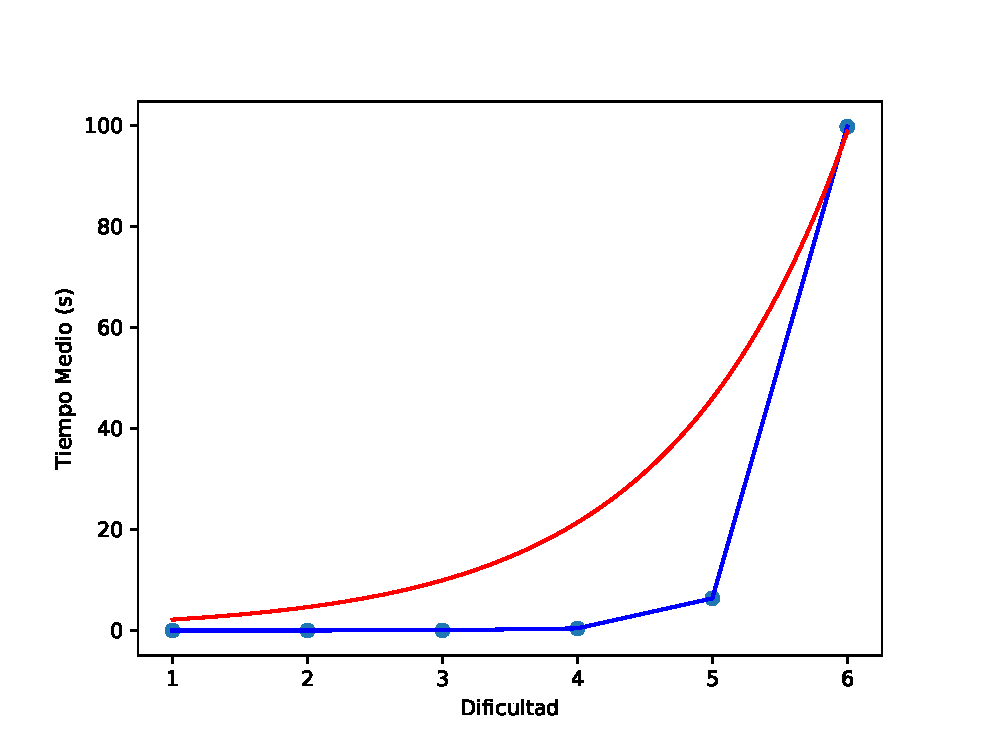
\includegraphics[width=12cm]{figures/resultados_pow.eps}
  \caption{Comparación entre los resultados y la función $y = 2^x$}
  \label{fig:resultados}
\end{figure}
En la figura \ref{fig:resultados} se aprecia que los resultados obtenidos tienen un comportamiento similar a la función $y(x) = 2^x$. Aunque esto no puede considerarse como una aproximación buena del algoritmo de prueba de trabajo con la función hash SHA-256, pues ni el tamaño de la muestra es lo suficientemente grande, ni se han hecho comprobaciones para dificultades superiores a 6, sí es un indicador de que este comportamiento es cuasi-exponencial.
%Implementaremos el algoritmo visto en \ref{chap3:pow}
%Uno de los problemas del algoritmo de prueba de trabajo del Bitcoin es que todo el esfuerzo en términos de procesamiento que se usa para resolver el puzzle es en esencia inútil (no es verdaderamente inútil, pues cumple la función para la que está diseñado...). Esto está detrás de las graves implicaciones medioambientales del Bitcoin y de otras populares criptomonedas (poner referencia y datos sobre el consumo energético). Lo que proponemos es utilizar los cálculos con las funciones hash en el algoritmo de prueba de trabajo para buscar colisiones en la función SHA-256, tal como se definieron en \ref{hash}
%\cleardoublepage

\chapter{Conclusiones}\label{conclusiones}
\section{Discusión plan de estudios}
En la realización de este trabajo han sido importantes los conocimientos adquiridos en las asignaturas de Álgebra Básica y Ecuaciones Algebraicas del plan de estudios de Matemáticas. El contenido de estas materias resultó esencial para entender las diversas cuestiones referentes a la criptografía tratadas en el capítulo \ref{cap1}. Sin embargo, todo lo relativo a curvas elípticas se estudia en la asignatura de Curvas Algebraicas, optativa del último curso del itinerario de Matemática Pura, que por tanto no es común a todos los estudiantes. Igualmente, no existe en la carrera ninguna asignatura donde se traten en profundidad la criptografía, que tal y como se ha visto no solo es un área de conocimiento fundamental en el desarrollo del Blockchain, sino que resulta fundamental en multitud de áreas de la economía, la ciencia o la industria y a su vez está conectada directamente con el álgebra.

Al problema del consenso tratado en \ref{cap4} se hace mención en la asignatura de Programación Paralela, optativa del itinerario de Ciencias de la Computación, pero no es este tema uno de los contenidos centrales de esta materia.

En lo referente a la implementación del protocolo blockchain han sido de gran importancia los conocimientos adquiridos en la asignatura de Informática de primer curso, sobre el lenguaje de programación Python. Han sido también de gran importancia la optativa de cuarto curso Programación Paralela, mencionada anteriormente, donde se estudian casos prácticos de sistemas distribuidos. Esto ha hecho posible construir la red p2p sobre la que se ha establecido la  implementación del protocolo Blockchain realizada en este trabajo. Al igual que no existe una asignatura donde se traten cuestiones teóricas referentes a la criptografía, tampoco existe una donde estas cuestiones se analicen desde un punto de vista más práctico, algo que también se ha echado en falta en el proceso de implementación, por lo que se ha tenido que recurrir a diferentes manuales y documentos mencionados en la bibliografía.  
\section{Ideas finales y posible trabajo futuro}
Este trabajo ha permitido desarrollar los conceptos fundamentales en los que se sustenta el protocolo Blockchain. Ha sido posible justificar su funcionamiento y corrección a partir de la teoría de curvas algebraicas, en particular del algoritmo ECDSA para la firma y verificación de mensajes, así como de las funciones hash. El interés despertado por esta tecnología en el último lustro se ha debido fundamentalmente a las oportunidades de negocio que han generado las criptomonedas. Por tanto una parte importante de los trabajos y documentos sobre el blockchain se han centrado en como generar valor a partir de este protocolo pasando por alto los aspectos teóricos que sustentan su funcionamiento. 
También suele ser común tratar los términos Blockchain y Bitcoin como sinónimos, esto además de no ser exacto, pues como hemos visto el Blockchain trasciende a esta criptomoneda, enturbia a este protocolo al vincularlo con ciertas actividades ilegales (o al menos alegales) que se han aprovechado del anonimato y seguridad que ofrece el Bitcoin.


Por otra parte se han conseguido explicar cuestiones generales sobre la especificación del Blockchain que resultan de utilidad en el estudio de aplicaciones de esta tecnología. Entender este protocolo como un mecanismo de consenso permite utilizarlo en la resolución de diversos problemas de la programación distribuida. Por último, la implementación del protocolo además de mostrar uno de los posibles usos que se le puede dar a esta tecnología prueba que llevar a la práctica las ideas básicas del Blockchainn es una tarea directa y sencilla.


Las reservas o temores de diversos organismos entre los que se encuentran los estados respecto a las criptomonedas están bien fundadas en la medida en que la estructura descentralizada de cadena de bloques anula el control de las entidades centrales sobre el sistema monetario. Pero más allá de las criptomonedas el Blockchain tiene el potencial para introducir transformaciones en diversos aspectos de la sociedad. Esta tecnología cambiará la forma de entender los contratos, las transacciones y en general todas las relaciones que requieren de cierta confianza entre las partes y que tradicionalmente han necesitado de la intervención de intermediarios que actúen como garantes del buen funcionamiento de tales actividades. En cualquier caso, hablar del Blockchain como una (o la) tecnología del futuro tampoco es exacto, porque ya es una tecnología del presente.


%Esta tecnología ha despertado un enorme interés en el último lustro y poder entender y justificar su funcionamiento resulta de gran importancia. La importancia de las funciones hash, y el 



%Las oportunidades de negocio que han generado las criptomonedas ha despertado el interés de las escuelas de negocio y facultades de economía, sin embargo el acercamiento de matemáticos y científicos de la computación al blockchain ha sido mucho más discreto. Por tanto, aún existen pocos artículos y trabajos teóricos sobre el tema.
%La teoría de curvas elípticas es un campo muy desarrollado y de gran importancia tanto en el álgebra como en la criptografía. 

%Más allá de las criptomonedas el blockchain tiene el potencial de introducir profundas transformaciones tanto económicas como sociales. Estas transformaciones

%Hablar del potencial del blockchain resulta contraproducente pues

%La trascendencia de esta tecnología va más allá de una aplicación ec

% +-------------------------------------------------------------------------+
% | References                                                              
% +--------------------------------------------------------------------+
% | This template uses the BibTeX program to format references.  The
% | 3 lines below create a separate Bibliography section and add
% | an entry for "Bibliography" to the Table of Contents.  The actual
% | data for your references (author, title, journal, date, etc.) are
% | entered in the references.bib file.  See that file for information
% | on how to enter references.
% +--------------------------------------------------------------------+

%\bibdata{references}
%\bibliography{references}
%\addcontentsline{toc}{chapter}{Bibliografía}
\begin{thebibliography}{10}
\bibitem{bitcoin}
S. Nakamoto, \textit{Bitcoin: A peer-to-peer electronic cash system}, 2008, \url{http://bitcoin.org/bitcoin.pdf}  Accessed: 2018-11-13. (Archived by WebCite at \url{http://www.webcitation.org/73uMoT8YE})

\bibitem[Hankerson, 2004]{elliptic_cripto}
  D. Hankerson, A. Menezes, S. Vanstone,
  \textit{Guide to Elliptic Curve Cryptography},
  \newline Springer, New York, NY,
  2nd edition,
  2004.
\bibitem[Cassels, J. (1991)]{group_law}
Cassels, J. (1991). 
\textit{Non-singular cubics. The group law. In LMSST: 24 Lectures on Elliptic Curves}
 (London Mathematical Society Student Texts, pp. 27-31). Cambridge: Cambridge University Press. doi:10.1017/CBO9781139172530.008
 
\bibitem[Verrill, H. (2000)]{group_law_verrill}
 H. Verrill, \textit{Group Law for elliptic Curves}, Lecture Notes \url{http://www.math.ku.dk/~kiming/lecture_notes/2000-2001-elliptic_curves/grouplaw.pdf} Accessed: 2018-11-13. (Archived by WebCite at \url{http://www.webcitation.org/73uN8g2Qm})
 
\bibitem[Kristin, 2009]{discrete_log}
K. Lauter, K. Stange, \textit{The Elliptic Curve Discrete Logarithm Problem and Equivalent Hard Problems for Elliptic Divisibility Sequences. Selected Areas in Cryptography} pp. 309-327, Springer Berlin Heidelberg, isbn 978-3-642-04159-4
 
%\bibitem{sha-256}\textit{Secure Hash Standard (SHS)} Information Technology Laboratory National Institute of Standards and Technology, 2015,  \url{https://nvlpubs.nist.gov/nistpubs/FIPS/NIST.FIPS.180-4.pdf} Accessed: 2018-11-13. (Archived by WebCite at \url{http://www.webcitation.org/73uNM08ZE}) 

\bibitem{sha-1} 
M. Stevens, E. Bursztein, P. Karpman, A. Albertini, Y. Markov, \textit{The first collision for full SHA-1}, Google Research, \url{http://shattered.io/static/shattered.pdf} Accessed: 2018-11-13. (Archived by WebCite at \url{http://www.webcitation.org/73uNS2E8T}) 
 
\bibitem[Tanenbaum, 2002]{distributed_system}
 A. Tanenbaum, M. van Steen. 
 \textit{Distributed Systems: Principles and Paradigms.} 2002.
 
\bibitem[Lamport, 2004]{2commit}L. Lamport, J. Gray, Consensus on transaction commit, Technical
Report MSR-TR-2003-96, Microsoft Research, January 2004.


\bibitem[A. Back, 2002]{hashcash} A. Back \textit{Hashcash - A Denial of Service Counter-Measure
},2002,\url{http://www.hashcash.org/papers/hashcash.pdf} Accessed: 2018-11-13. (Archived by WebCite at \url{http://www.webcitation.org/73uNgCTaA})

\bibitem[R. Wattenhofer, 2016]{blockchain science} 
R. Wattenhofer, \textit{The Science of the Blockchain.},2016, Inverted Forest Publishing.

\bibitem{electricidad} \textit{Bitcoin Mining Now Consuming More Electricity Than 159 Countries Including Ireland \& Most Countries In Africa} \url{https://powercompare.co.uk/bitcoin/} Accessed: 2018-11-13. (Archived by WebCite at \url{http://www.webcitation.org/73uNlJOrn})

\bibitem{pos} \textit{Proof of Stake FAQ} \url{https://github.com/ethereum/wiki/wiki/Proof-of-Stake-FAQ#what-is-proof-of-stake} Accessed: 2019-02-19. (Archived by WebCite at \url{http://www.webcitation.org/76JNGcsPi})

\bibitem{pob} \textit{Slimcoin
A Peer-to-Peer Crypto-Currency with Proof-of-Burn}, 2014  \url{http://www.doc.ic.ac.uk/~ids/realdotdot/crypto_papers_etc_worth_reading/proof_of_burn/slimcoin_whitepaper.pdf} Accessed: 2019-02-19. (Archived by WebCite at \url{http://www.webcitation.org/76JMlsixP})

\bibitem[Lamport, 1982]{byzantine generals}
L. Lamport , R. Shostak , M. Pease, \textit{The Byzantine Generals Problem}, 1982,  ACM Transactions on Programming Languages and Systems, pp. 1-2 \url{https://web.archive.org/web/20170205142845/http://lamport.azurewebsites.net/pubs/byz.pdf} Accessed: 2019-02-19. (Archived by WebCite at \url{http://www.webcitation.org/76JN02lQC})

\bibitem[V. Gramoli, 2017]{blockchain consensus}
V. Gramoli, \textit{From blockchain consensus back to byzantine consensus.} (2017).  
\url{http://poseidon.it.usyd.edu.au/~gramoli/web/doc/pubs2/Blockchain2Byzantine.pdf} Accessed: 2019-02-19. (Archived by WebCite at \url{http://www.webcitation.org/76JN3x2HG})

\bibitem{paxos} L. Lamport, \textit{Paxos Made Simple}, 2001, \url{http://lamport.azurewebsites.net/pubs/paxos-simple.pdf} Accessed: 2019-02-20. (Archived by WebCite at \url{http://www.webcitation.org/76KrEjmMl})

\bibitem{raft} \textit{Raft consensus algorithm} \url{https://raft.github.io/} Accessed: 2019-02-20. (Archived by WebCite at \url{http://www.webcitation.org/76Kr1hHPJ})

\bibitem{fastecdsa} Documentación librería fastecdsa \url{https://pypi.org/project/fastecdsa/} Accessed: 2018-11-13. (Archived by WebCite at \url{http://www.webcitation.org/73uOA1nmI})

\bibitem{hashlib} Documentación librería hashlib de Python \url{https://docs.python.org/2/library/hashlib.html} Accessed: 2018-11-13. (Archived by WebCite at \url{http://www.webcitation.org/73uO4Hti7})

\bibitem{multiprocessing} Documentación librería multiprocessing \url{https://docs.python.org/2/library/multiprocessing.html} Accessed: 2018-11-13. (Archived by WebCite at \url{http://www.webcitation.org/73uNs8AP7})

\end{thebibliography}

%\begin{thebibliography}{12}

%\bibitem{elliptic_cripto}
%  D. Hankerson, A.Menezes, S.Vanstone,
%  \textit{Guide to Elliptic Curve Cryptography},
%  Springer, New York, NY,
%  2nd edition,
%  2004.



%\end{thebibliography}
%\addcontentsline{toc}{chapter}{Bibliografía}
% +--------------------------------------------------------------------+
% | Finally, we generate the appendix.  To add or delete appendices,
% | add or remove the line
% |
% |     \input{appendixX.tex}
% |
% | where "X" is the letter designation of the Appendix (A, B, C, etc.)
% | You should have one \input{appendixX.tex} line and a corresponding
% | file appendixX.tex for each appendix.                                 |
% +--------------------------------------------------------------------+

%\appendix

%% +--------------------------------------------------------------------+
% | Appendix B Page (Optional)                                         |
% +--------------------------------------------------------------------+

\cleardoublepage

\chapter{Título para este segundo apéndice}
\label{Appendix:Key2}

% +--------------------------------------------------------------------+
% | Enter text for your Appendix page in the space below this box.     |
% |                                                                    |
% +--------------------------------------------------------------------+


\end{document}
